
\documentclass[aspectratio=169,xcolor=dvipsnames]{beamer}
%\usetheme{SimplePlus}

\usepackage{hyperref}
\usepackage{graphicx} % Allows including images
%usepackage{booktabs} % Allows the use of \toprule, \midrule and \bottomrule in tables
\usepackage{tabularx}

\title[short title]{Prosessdynamikk og PID-tuning} % The short title appears at the bottom of every slide, the full title is only on the title page
%\subtitle{Subtitle}

\author[Fred-Olav] {Fred-Olav Mosdal}

\institute[Gand VGS]{} % Your institution as it will appear on the bottom of every slide, may be shorthand to save space
\date{\today} % Date, can be changed to a custom date

\begin{document}
%\chapter{Process dynamics and PID controller tuning}
%
%To \textit{tune} a feedback control system means to adjust parameters in the controller to achieve robust control over the process.  ``Robust'' in this context is usually defined as stability of the process variable despite changes in load, fast response to changes in setpoint, minimal oscillation following either type of change, and minimal offset (error between setpoint and process variable) over time.
%
%``Robust control'' is far easier to define than it is to achieve.  With PID (Proportional-Integral-Derivative) control being the most common feedback control algorithm used in industry, it is important for all instrumentation practitioners to understand how to tune these controllers effectively and with a minimum investment of time.
%
%\vskip 10pt
%
%Different types of processes, having different dynamic (time-dependent) behaviors, require different levels of proportional, integral, and derivative control action to achieve stability and robust response.  It is therefore imperative for anyone seeking to tune a PID controller to understand the dynamic nature of the process being controlled.  For this reason, the chapter begins with an exploration of common process characteristics before introducing techniques useful in choosing practical P, I, and D tuning parameter values.
%
%
%
%
%
%
%
%
%\filbreak
%\section{Process characteristics}
%
%\label{process_characteristics}
%
%Perhaps the most important rule of controller tuning is to \textit{know the process before attempting to adjust the controller's tuning}.  Unless you adequately understand the nature of the process you intend to control, you will have little hope in actually controlling it well.  This section of the book is dedicated to an investigation of different process characteristics and how to identify each.  
%
%Quantitative PID tuning methods (see section \ref{quantitative_pid_tuning} beginning on page \pageref{quantitative_pid_tuning}) attempt to map the characteristics of a process so good PID parameters may be chosen for the controller.  The goal of this section is for you to understand various process types by observation and qualitative analysis so you may comprehend why different tuning parameters are necessary for each type, rather than mindlessly following a step-by-step PID tuning procedure.
%
%\vskip 10pt
%
%The three major classifications of process response are \textit{self-regulating}, \textit{integrating}, and \textit{runaway}.  Each of these process types is defined by its response to a step-change in the manipulated variable (e.g. control valve position or state of some other final control element).  A ``self-regulating'' process responds to a step-change in the final control element's status by settling to a new, stable value.  An ``integrating'' process responds by ramping either up or down at a rate proportional to the magnitude of the final control element's step-change.  Finally, a ``runaway'' process responds by ramping either up or down at a rate that increases over time, headed toward complete instability without some form of corrective action from the controller.
%
%Self-regulating, integrating, and runaway processes have very different control needs.  PID tuning parameters that may work well to control a self-regulating process, for example, will \textit{not} work well to control an integrating or runaway process, no matter how similar any of the other characteristics of the processes may be\footnote{To illustrate, self-regulating processes require significant integral action from a controller in order to avoid large offsets between PV and SP, with minimal proportional action and no derivative action.  Integrating processes, in contrast, may be successfully controlled primarily on proportional action, with minimal integral action to eliminate offset.  Runaway processes absolutely require derivative action for dynamic stability, but derivative action alone is not enough: some integral action will be necessary to eliminate offset.  Even if knowledge of a process's dominant characteristic does not give enough information for us to quantify P, I, or D values, it will tell us which tuning constant will be most important for achieving stability.}.  By first identifying the characteristics of a process, we may draw some general conclusions about the P, I, and D setting values necessary to control it well.
%
%\vskip 10pt
%
%Perhaps the best method for testing a process to determine its natural characteristics is to place the controller in \textit{ manual mode} and introduce a step-change to the controller output signal.  It is critically important that the loop controller be in manual mode whenever process characteristics are being explored.  If the controller is left in the automatic mode, the response seen from the process to a setpoint or load change will be partly due to the natural characteristics of the process itself \textit{and} partly due to the corrective action of the controller.  The controller's corrective action thus interferes with our goal of exploring process characteristics.  By placing the controller in ``manual'' mode, we turn off its corrective action, effectively removing its influence by breaking the feedback loop between process and controller, controller and process.  In manual mode, the response we see from the process to an output (manipulated variable) or load change is \textit{purely} a function of the natural process dynamics, which is precisely what we wish to discern.
%
%A test of process characteristics with the loop controller in manual mode is often referred to as an \textit{open-loop} test, because the feedback loop has been ``opened'' and is no longer a complete loop.  Open-loop tests are the fundamental diagnostic technique applied in the following subsections.  \index{Open-loop test}  \index{Characterizing process dynamics}
%
%
%
%
%
%
%
%
%
%\filbreak
%\subsection{Self-regulating processes}
%
%\label{self-regulating_processes}
%
%% ADD: sometimes called ``resistive'' processes
%
%If a liquid flow-control valve is opened in a step-change fashion, flow through the pipe tends to self-stabilize at a new rate very quickly.  The following illustration shows a typical liquid flow-control installation, with a process trend showing the flow response following a manual-mode (also known as ``open-loop'') step-change in valve position:  \index{Self-regulating process}  \index{Open-loop test}
% 
\begin{frame}
	\frametitle{Selvregulerende prosess}

	$$\includegraphics[width=1\textwidth]{process_01.eps}$$
\end{frame}

%$$\includegraphics{process_01.eps}$$
%
%The defining characteristic of a self-regulating process is its inherent ability to settle at a new process variable value without any corrective action on the part of the controller.  In other words, a self-regulating process will exhibit a unique process variable value for each possible output (valve) value.  The inherently fast response of a liquid flow control process makes its self-regulating nature obvious: the self-stabilization of flow generally takes place within a matter of seconds following the valve's motion.  Many other processes besides liquid flow are self-regulating as well, but their slow response times require patience on the part of the observer to tell that the process will indeed self-stabilize following a step-change in valve position.
%
%A corollary to the principle of self-regulation is that a unique output value \textit{will be required} to achieve a new process variable value.  For example, to achieve a greater flow rate, the control valve must be opened further and held at that further-open position for as long as the greater flow rate is desired.  This presents a fundamental problem for a proportional-only controller.  Recall the formula for a proportional-only controller, defining the output value ($m$) by the error ($e$) between process variable and setpoint multiplied by the gain ($K_p$) and added to the bias ($b$):
%
%$$m = K_p e + b$$
%
%\noindent
%Where,
%
%$m$ = Controller output
%
%$e$ = Error (difference between PV and SP)
%
%$K_p$ = Proportional gain
%
%$b$ = Bias
%
%\vskip 10pt
%
%Suppose we find the controller in a situation where there is no error (PV = SP), and the flow rate is holding steady at some value.  If we then increase the setpoint value (calling for a greater flow rate), the error will increase, driving the valve further open.  As the control valve opens further, flow rate naturally increases to match.  This increase in process variable drives the error back toward zero, which in turn causes the controller to decrease its output value back toward where it was before the setpoint change.  However, the error can never go all the way back to zero because if it did, the valve would return to its former position, and that would cause the flow rate to self-regulate back to its original value before the setpoint change was made.  What happens instead is that the control valve begins to close as flow rate increases, and eventually the process finds some equilibrium point where the flow rate is steady at some value less than the setpoint, creating just enough error to drive the valve open just enough to maintain that new flow rate.  Unfortunately, due to the need for an error to exist, this new flow rate will fall shy of our setpoint.  We call this error \textit{proportional-only offset}, or \textit{droop}, and it is an inevitable consequence of a proportional-only controller attempting to control a self-regulating process. \index{Proportional-only offset} \index{Droop}
%
%For any fixed bias value, there will be only one setpoint value that is perfectly achievable for a proportional-only controller in a self-regulating process.  Any other setpoint value will result in some degree of offset in a self-regulating process.  If dynamic stability is more important than absolute accuracy (zero offset) in a self-regulating process, a proportional-only controller may suffice.  A great many self-regulating processes in industry have been and still are controlled by proportional-only controllers, despite some inevitable degree of offset between PV and SP.
%
%The amount of offset experienced by a proportional-only controller in a self-regulating process may be minimized by increasing the controller's gain.  If it were possible to increase the gain of a proportional-only controller to infinity, it would be able to achieve any setpoint desired with zero offset!  However, there is a practical limit to the extent we may increase the gain value, and that limit is \textit{oscillation}.  If a controller is configured with too much gain, the process variable will begin to oscillate over time, never stabilizing at any value at all, which of course is highly undesirable for any automatic control system.  Even if the gain is not great enough to cause sustained oscillations, excessive values of gain will still cause problems by causing the process variable to oscillate with decreasing amplitude for a period of time following a sudden change in either setpoint or load.  Determining the optimum gain value for a proportional-only controller in a self-regulating process is, therefore, a matter of compromise between excessive offset and excessive oscillation.
%
%\vskip 10pt
%
%Recall that the purpose of integral (or ``reset'') control action was the elimination of offset.  Integral action works by ramping the output of the controller at a rate determined by the magnitude of the offset: the greater the difference between PV and SP for an integral controller, the faster that controller's output will ramp over time.  In fact, the output will stabilize at some value \textit{only} if the error is diminished to zero (PV = SP).  In this way, integral action works tirelessly to eliminate offset.
%
%It stands to reason then that a self-regulating process \textit{absolutely requires} some amount of integral action in the controller in order to achieve zero offset for all possible setpoint values.  The more aggressive (faster) a controller's integral action, the sooner offset will be eliminated.  Just how much integral action a self-regulating process can tolerate depends on the magnitudes of any time lags in the system.  The faster a process's natural response is to a manual step-change in controller output, the better it will respond to aggressive integral controller action once the controller is placed in automatic mode.  Aggressive integral control action in a slow process, however, will result in oscillation due to integral wind-up\footnote{Recall that wind-up is what happens when integral action ``demands'' more from a process than the process can deliver.  If integral action is too aggressive for a process (i.e. fast integral controller action in a process with slow time lags), the output will ramp too quickly, causing the process variable to overshoot setpoint which then causes integral action to wind the other direction.  As with proportional action, too much integral action will cause a self-regulating process to oscillate.}.  \index{Wind-up, controller} \index{Integral windup} \index{Reset windup}
%
%It is not uncommon to find self-regulating processes being controlled by \textit{integral-only} controllers.  An ``integral-only'' process controller is an instrument lacking proportional or derivative control modes.  Liquid flow control is a nearly ideal candidate process for integral-only control action, due to its self-regulating and fast-responding nature.
%
%\vskip 10pt
%
%\noindent
%\textbf{Summary:}
%
%\begin{itemize}
%\item Self-regulating processes are characterized by their natural ability to stabilize at a new process variable value following changes in the control element value or load(s).
%\item Self-regulating processes \textit{absolutely require} integral controller action to eliminate offset between process variable and setpoint, because only integral action is able to create a different controller output value once the error returns to zero.
%\item Faster integral controller action results in quicker elimination of offset.
%\item The amount of integral controller action tolerable in a self-regulating process depends on the degree of time lag in the system.  Too much integral action will result in oscillation, just like too much proportional control action.
%\end{itemize}
%
%
%
%
%
%\filbreak
%\subsection{Integrating processes}
%
%\label{integrating_processes}
%
%% ADD: sometimes called ``capacitive'' processes
%
%A good example of an integrating process is liquid level control, where either the flow rate of liquid into or out of a vessel is constant and the other flow rate varies.  If a control valve is opened in a step-change fashion, liquid level in the vessel ramps at a rate proportional to the difference in flow rates in and out of the vessel.  The following illustration shows a typical liquid level-control installation, with a process trend showing the level response to a step-change in valve position (with the controller in manual mode, for an ``open-loop'' test):  \index{Integrating process}  \index{Open-loop test}
%
\begin{frame}
	\frametitle{Integrerende prosess}

	$$\includegraphics[width=1\textwidth]{process_02.eps}$$
\end{frame}

%$$\includegraphics{process_02.eps}$$
%
%It is critically important to realize that this ramping action of the process variable over time is a characteristic of the process itself, not the controller.  When liquid flow rates in and out of a vessel are mis-matched, the liquid level within that vessel will change at a rate proportional to the difference in flow rates.  The trend shown here reveals a fundamental characteristic of the process, not the controller (this should be obvious once it is realized that the step-change in output is something that would only ever happen with the controller in \textit{manual} mode).
%
%Mathematically, we may express the integrating nature of this process using calculus notation.  First, we may express the \textit{rate of change} of volume in the tank over time ($dV \over dt$) in terms of the flow rates in and out of the vessel:
%
%$${dV \over dt} = Q_{in} - Q_{out}$$
%
%For example, if the flow rate of liquid going into the vessel was 450 gallons per minute, and the constant flow rate drawn out of the vessel was 380 gallons per minute, the volume of liquid contained within the vessel would increase over time at a rate equal to 70 gallons per minute: the difference between the in-flow and the out-flow rates.
%
%Another way to express this mathematical relationship between flow rates and liquid volume in the vessel is to use the calculus function of \textit{integration}:
%
%$$\Delta V = \int_0^T (Q_{in} - Q_{out}) \> dt$$
%
%The amount of liquid volume accumulated in the vessel ($\Delta V$) between time 0 and time $T$ is equal to the sum ($\int$) of the products (multiplication) of difference in flow rates in and out of the vessel ($Q_{in} - Q_{out}$) during infinitesimal increments of time ($dt$).
%
%In the given scenario of a liquid level control system where the out-going flow is held constant, this means the level will be stable only at one in-coming flow rate (where $Q_{in} = Q_{out}$).  At any other controlled flow rate, the level will either be increasing over time or decreasing over time.
%
%This process characteristic perfectly matches the characteristic of a proportional-only controller, where there is one unique output value when the error is zero (PV = SP).  We may illustrate this by performing a ``thought experiment'' on the liquid level-control process shown earlier having a constant draw out the bottom of the vessel.  Imagine this process controlled by a proportional-only controller in automatic mode, with the bias value ($b$) of the controller set to the exact value needed by the control valve to make in-coming flow exactly equal to the constant out-going flow (draw).  This means that when the process variable is precisely equal to setpoint (PV = SP), the in-flow will match the out-flow and therefore the liquid level will hold constant.  If now an operator were to increase the setpoint value (with the controller in automatic mode), it will cause the valve to open further, adding liquid at a faster rate to the vessel.  The naturally integrating nature of the process will result in an increasing liquid level.  As level increases, the amount of error in the controller decreases, causing the valve to approach its original (bias) position.  When the level reaches the new setpoint, proportional-only action will return the controller output to its original (bias) value, thus returning the in-flow control valve to its original position.  This return to the bias position makes in-flow once again equal to out-flow, and so the level remains constant at the new setpoint with absolutely no offset (``droop'') even though the controller only exhibits proportional action.  Proportional-only offset exists in a self-regulating process because a new valve position is needed to achieve any new setpoint value.  Proportional-only offset does not occur on setpoint changes in an integrating process because only one valve position is needed to hold the process variable constant at \textit{any} setpoint value.  \index{Thought experiment}  \index{Problem-solving technique: thought experiment}
%
%The more aggressive the controller's proportional action, the sooner the integrating process will reach new setpoints.  Just how much proportional action (gain) an integrating process can tolerate depends on the magnitudes of any time lags in the system as well as the magnitude of noise in the process variable signal.  Any process system with time lags will oscillate if the controller has sufficient gain.  Noise is a problem because proportional action directly reproduces process variable noise on the output signal: too much gain, and just a little bit of PV noise translates into a control valve whose stem position constantly jumps around.
%
%Purely integrating processes do not require integral control action to eliminate offset as is the case with self-regulating processes, following a setpoint change.  The natural integrating action of the process eliminates offset that would otherwise arise from setpoint changes.  More than that, the presence of any integral action in the controller will actually force the process variable to overshoot setpoint following a setpoint change in a purely integrating process!  Imagine a controller with integral action responding to a step-change in setpoint for the liquid level control process shown earlier.  As soon as an error develops, the integral action will begin ``winding up'' the output value, forcing the valve to open more than proportional action alone would demand.  By the time the liquid level reaches the new setpoint, the valve will have reached a position greater than where it originally was before the setpoint change\footnote{In a proportional-only controller, the output is a function of error (PV $-$ SP) and bias.  When PV = SP, bias alone determines the output value (valve position).  However, in a controller with integral action, the zero-offset output value is determined by \textit{how long} and \textit{how far} the PV has previously strayed from SP.  In other words, there is no fixed bias value anymore.  Thus, the output of a controller with integral action will \textit{not} return to its previous value once the new SP is reached.  In a purely integrating process, this means the PV will \textit{not} reach stability at the new setpoint, but will continue to rise until all the ``winding up'' of integral action is un-done.}, which means the liquid level will \textit{not} stop rising when it reaches setpoint, but in fact will overshoot setpoint.  Only after the liquid level has spent sufficient time above setpoint will the integral action of the controller ``wind'' back down to its previous level, allowing the liquid level to finally achieve the new setpoint.
%
%This is not to say that integral control action is completely unnecessary in integrating processes -- far from it.  If the integrating process is subject to \textit{load} changes, only integral action can return the PV back to the SP value (eliminate offset).  Consider, in our level control example, if the out-going flow rate were to change.  Now, a new valve position will be required to achieve stable (unchanging) level in the vessel.  A proportional-only controller is able to generate a new valve position \textit{only} if an error develops between PV and SP.  Without at least some degree of integral action configured in the controller, that error will persist indefinitely.  Or consider if the liquid supply pressure upstream of the control valve were to change, resulting in a different rate of incoming flow for the same valve stem position as before.  Once again, the controller would have to generate a different output value to compensate for this process change and stabilize liquid level, and the only way a proportional-only controller could do that is to let the process variable drift a bit from setpoint (the definition of an error or offset). 
%
%\vskip 10pt
%
%The example of an integrating process used here is just one of many possible processes where we are dealing with either a \textit{mass balance} or an \textit{energy balance} problem.  ``Mass balance'' is the accounting of all mass into and out of a process.  Since the Law of Mass Conservation states the impossibility of mass creation or destruction, all mass into and out of a process must be accounted for.  If the mass flow rate into a process does not equal the mass flow rate out of a process, the process must be either gaining or losing an internal store of mass.  The same may be said for energy: all energy flowing into and out of a process must be accounted for, since the Law of Energy Conservation states the impossibility of energy creation or destruction.  If the energy flow rate (input power) into a process does not equal the energy flow rate (output power) out of a process, the process must be either gaining or losing an internal store of energy.  \index{Mass balance}  \index{Energy balance}    \index{Conservation of Mass}  \index{Conservation of Energy}
%
%\filbreak
%
%$$\includegraphics{process_32.eps}$$
%
%Common examples of integrating processes include the following:
%
%\begin{itemize}
%\item Liquid level control -- \textit{mass balance} -- when the flow of liquid either into or out of a vessel is manipulated, and the other flows in or out of the vessel are constant
%\item Gas pressure control -- \textit{mass balance} -- when the flow of gas either into or out of a vessel is manipulated, and the other flows in or out of the vessel are constant
%\item Storage bin level control -- \textit{mass balance} -- when the conveyor feed rate into the bin is manipulated, and the draw from the bin is constant
%\item Temperature control -- \textit{energy balance} -- when the flow of heat into or out of a process is manipulated, and all other heat flows are constant
%\item Speed control -- \textit{energy balance} -- when the force (linear) or torque (angular) applied to a mass is manipulated, and all other loads are constant in force or torque
%\end{itemize}
%
%In a self-regulating process, the control element (valve) exerts control over \textit{both} the in-flow and the out-flow of either mass or energy.  In the previous subsection, where liquid flow control was the process example, the mass balance consisted of liquid flow into the valve and liquid flow out of the valve.  Since the piping was essentially a ``series'' path for an incompressible fluid, where input flow must equal output flow at any given time, mass in and mass out were \textit{guaranteed} to be in a state of balance, with one valve controlling both.  This is why a change in valve position resulted in an almost immediate change and re-stabilization of flow rate: the valve exerts immediate control over both the incoming and the outgoing flow rates, with both in perfect balance.  Therefore, nothing ``integrates'' over time in a liquid flow control process because there can never be an imbalance between in-flow and out-flow.
%
%In an integrating process, the control element (valve) exerts control over \textit{either} the in-flow \textit{or} the out-flow of mass or energy, but never both.  Thus, changing valve position in an integrating process causes an imbalance of mass flow and/or energy flow, resulting in the process variable ramping over time as either mass or energy accumulates in (or depletes from) the process.
%
%\filbreak
%
%Our ``simple'' example of an integrating (level-control) process becomes a bit more complicated if the outgoing flow depends on level, as is the case with a gravity-drained vessel where the outgoing flow is a function of liquid level in the vessel rather than being fixed at a constant rate as it was in the previous example:
%
%$$\includegraphics{process_03.eps}$$
%
%If we subject the control valve to a manual step-change increase, the flow rate of liquid into the vessel immediately increases.  This causes an imbalance of incoming and outgoing flow, resulting in the liquid level rising over time.  As level rises, however, increasing hydrostatic pressure across the manual valve at the vessel outlet causes the outgoing flow rate to increase.  This causes the mass imbalance rate to be less than it was before, resulting in a decreased integration rate (rate of level rise).  Thus, the liquid level still rises, but at a slower and slower rate as time goes on.  Eventually, the liquid level will become high enough that the pressure across the manual valve forces a flow rate out of the vessel equal to the flow rate into the vessel.  At this point, with matched flow rates, the liquid level stabilizes with no corrective action from the controller (remember, the step-change in output was made in manual mode!).  Note the final result of letting the outgoing flow be a function of liquid level: \textit{what used to be an integrating process has now become a self-regulating process,} albeit one with a substantial lag time.
%
%Many processes ideally categorized as integrating actually behave in this manner.  Although the manipulated variable may control the flow rate into or out of a process, the other flow rates often change with the process variable.  Returning to our list of integrating process examples, we see how a PV-variable load in each case can make the process self-regulate:
%
%\begin{itemize}
%\item Liquid level control -- \textit{mass balance} -- if the in-flow naturally decreases as liquid level rises and/or the out-flow naturally increases as liquid level rises, the vessel's liquid level will tend to self-regulate instead of integrate
%\item Gas pressure control -- \textit{mass balance} -- if in-flow naturally decreases as pressure rises and/or the out-flow naturally increases as pressure rises, the vessel's pressure will tend to self-regulate instead of integrate
%\item Storage bin level control -- \textit{mass balance} -- if the draw from the bin increases with bin level (greater weight pushing material out at a faster rate), the bin's level will tend to self-regulate instead of integrate
%\item Temperature control -- \textit{energy balance} -- if the process naturally loses heat at a faster rate as temperature increases and/or the process naturally takes in less heat as temperature rises, the temperature will tend to self-regulate instead of integrate 
%\item Speed control -- \textit{energy balance} -- if drag forces on the object increase with speed (as they usually do for any fast-moving object), the speed will tend to self-regulate instead of integrate
%\end{itemize}
%
%We may generalize all these examples of integrating processes turned self-regulating by noting the one aspect common to all of them: some natural form of \textit{negative feedback} exists internally to bring the system back into equilibrium.  In the mass-balance examples, the physics of the process ensure a new balance point will eventually be reached because the in-flow(s) and/or out-flow(s) naturally change in ways that oppose any change in the process variable.  In the energy-balance examples, the laws of physics again conspire to ensure a new equilibrium because the energy gains and/or losses naturally change in ways that oppose any change in the process variable.  The presence of a control system is, of course, the ultimate example of negative feedback working to stabilize the process variable.  However, the control system may not be the \textit{only} form of negative feedback at work in a process.  All self-regulating processes are that way because they intrinsically possess some degree of negative feedback acting as a sort of natural, proportional-only control system.  \index{Negative feedback}
%
%\filbreak
%
%This one detail completely alters the fundamental characteristic of a process from integrating to self-regulating, and therefore changes the necessary controller parameters.  Self-regulation guarantees at least some integral controller action is \textit{necessary} to attain new setpoint values.  A purely integrating process, by contrast, requires no integral controller action at all to achieve new setpoints, and in fact is \textit{guaranteed} to suffer overshoot following setpoint changes if the controller is programmed with any integral action at all!  Both types of processes, however, need some amount of integral action in the controller in order to recover from \textit{load} changes.
%
%\vskip 10pt
%
%\noindent
%\textbf{Summary:}
%
%\begin{itemize}
%\item Integrating processes are characterized by a ramping of the process variable in response to a step-change in the control element value or load(s).
%\item This integration occurs as a result of either \textit{mass flow imbalance} or \textit{energy flow imbalance} in and out of the process.
%\item Integrating processes are ideally controllable with proportional controller action alone.
%\item Integral controller action guarantees setpoint overshoot in a purely integrating process.
%\item Some integral controller action will be required in integrating processes to compensate for load changes.
%\item The amount of proportional controller action tolerable in an integrating process depends on the degree of time lag and process noise in the system.  Too much proportional action will result in oscillation (time lags) and/or erratic control element motion (noise).
%\item An integrating process will become self-regulating if sufficient negative feedback is naturally introduced.  This usually takes the form of loads varying with the process variable.
%\end{itemize}
%
%
%
%
%
%
%\filbreak
%\subsection{Runaway processes}
%
%A classic ``textbook'' example of a runaway process is an inverted pendulum: a vertical stick balanced on its end by moving the bottom side-to-side.  Inverted pendula are typically constructed in a laboratory environment by fixing a stick to a cart by a pivot, then equipping the cart with wheels and a reversible motor to give it lateral control ability.  A sensor (usually a potentiometer) detects the stick's angle from vertical, reporting that angle to the controller as the process variable.  The cart's motor is the final control element:   \index{Runaway process}
%
%$$\includegraphics{process_04.eps}$$
%
%The defining characteristic of a runaway process is its tendency to accelerate away from a condition of stability with no corrective action applied.  Viewed on a process trend, a runaway process tends to respond as follows to an open-loop step-change:  \index{Open-loop test}
%
%$$\includegraphics{process_05.eps}$$
%
%A synonym for ``runaway'' is \textit{negative self-regulation} or \textit{negative lag}, because the process variable curve over time for a runaway process resembles the mathematical inverse of a self-regulating curve with a lag time: it races away from the horizontal, while a self-regulating process variable draws closer and closer to the horizontal over time.  \index{Negative self-regulation}  \index{Negative lag}
%
%The ``Segway$^{TM}$'' personal transport device is a practical example of an inverted pendulum, with wheel motion controlled by a computer attempting to maintain the body of the vehicle in a vertical position.  As the human rider leans forward, it causes the controller to spin the wheels with just the right amount of acceleration to maintain balance.  There are many examples of runaway processes in motion-control applications, especially automated controls for vertical-flight vehicles such as helicopters and vectored-thrust aircraft such as the Harrier military fighter jet.  \index{Harrier jet airplane}  \index{Segway personal transport}
%
%Some chemical reaction processes are runaway as well, especially \textit{exothermic} (heat-releasing) reactions.  Most chemical reactions increase in rate as temperature rises, and so exothermic reactions tend to accelerate with time (either becoming hotter or becoming colder) unless checked by some external influence.  This poses a significant challenge to process control, as many exothermic reactions used to manufacture products must be temperature-controlled to ensure efficient production of the desired product.  Off-temperature chemical reactions may not ``favor'' production of the desired products, producing unwanted byproducts and/or failing to efficiently consume the reactants.  Furthermore, safety concerns usually surround exothermic chemical reactions, as no one wants their process to melt down or explode.
%
%What makes a runaway process behave as it does is internal \textit{positive feedback}.  In the case of the inverted pendulum, gravity works to pull an off-center pendulum even farther off center, accelerating it until it falls down completely.  In the case of exothermic chemical reactions, the direct relationship between temperature and reaction rate forms a positive feedback loop: the hotter the reaction, the faster it proceeds, releasing even more heat, making it even hotter.  It should be noted that \textit{endothermic} chemical reactions (absorbing heat rather than releasing heat) tend to be self-regulating for the exact same reason exothermic reactions tend to be runaway: reaction rate usually has a positive correlation with reaction temperature.  \index{Positive feedback}
%
%It is easy to demonstrate for yourself how challenging a runaway process can be to control.  Simply try to balance a long stick vertically in the palm of your hand.  You will find that the only way to maintain stability is to react swiftly to any changes in the stick's angle -- essentially applying a healthy dose of \textit{derivative} control action to counteract any motion from vertical.
%
%Fortunately, runaway processes are less common in the process industries.  I say ``fortunately'' because these processes are notoriously difficult to control and usually pose more danger than inherently self-regulating processes.  Many runaway processes are also nonlinear, making their behavior less intuitive to human operators.  
%
%\vskip 10pt
%
%\filbreak
%
%Just as integrating processes may be forced to self-regulate by the addition of (natural) negative feedback, intrinsically runaway processes may also be forced to self-regulate given the presence of sufficient natural negative feedback.  An interesting example of this is a pressurized water nuclear fission reactor.  \index{Negative feedback}
%
%Nuclear fission is a process by which the nuclei of specific types of atoms (most notably uranium-235 and plutonium-239) undergo spontaneous disintegration upon the absorption of an extra neutron, with the release of significant thermal energy and additional neutrons.  A quantity of fissile material such as $^{235}$U or $^{239}$Pu is subjected to a source of neutron particle radiation, which initiates the fission process, releasing massive quantities of heat which may then be used to boil water into steam and drive steam turbine engines to generate electricity.  The ``chain reaction'' of neutrons splitting fissile atoms, which then eject more neutrons to split more fissile atoms, is inherently exponential in nature.  The more atoms split, the more neutrons are released, which then proceed to split even more atoms.  The rate at which neutron activity within a fission reactor grows or decays over time is determined by the \textit{multiplication factor}\footnote{When a nucleus of uranium or plutonium undergoes fission (``splits''), it releases more neutrons capable of splitting additional uranium or plutonium nuclei.  The ratio of new nuclei ``split'' versus old nuclei ``split'' is the multiplication factor.  If this factor has a value of one (1), the chain reaction will sustain at a constant power level, with each new generation of atoms ``split'' equal to the number of atoms ``split'' in the previous generation.  If this multiplication factor exceeds unity, the rate of fission will increase over time.  If the factor is less than one, the rate of fission will decrease over time.  Like an inverted pendulum, the chain reaction has a tendency to ``fall'' toward infinite activity or toward no activity, depending on the value of its multiplication factor.}, and this factor is easily controlled by the insertion of neutron-absorbing \textit{control rods} into the reactor core.  \index{Fission, nuclear}  \index{Nuclear fission reactor}  \index{Multiplication factor, nuclear fission}
%
%Thus, a fission chain-reaction naturally behaves as an inverted pendulum.  If the multiplication factor is greater than 1, the reaction grows exponentially.  If the multiplication factor is less than 1, the reaction dies exponentially.  In the case of a nuclear weapon, the desired multiplication factor is as large as physically possible to ensure explosive reaction growth.  In the case of an operating nuclear power plant, the desired multiplication factor is exactly 1 to ensure stable power generation.
%
%\filbreak
%
%A simplified diagram of a pressurized-water reactor (PWR) is shown here:
%
%$$\includegraphics{process_31.eps}$$
%
%Water under high pressure (too high of pressure to boil) circulates through the reactor vessel, carrying heat away from the nuclear core, then transferring the heat energy to a heat exchanger (``steam generator'') where a second water loop is allowed to boil into steam and drive turbine engines to spin electrical generators.  Control rods inserted into the core by linear actuators adjust the multiplication factor of the reactor.
%
%If the multiplication factor of a fission reactor were solely controlled by the positions of these control rods, it would be a classic ``runaway'' process, with the reactor's power level tending to increase toward infinity or decrease toward zero if the rods were at any position other than one yielding a multiplication factor of precisely unity (1).  This would make nuclear reactors extremely difficult (if not impossible) to safely control.  Fortunately, there are ways to engineer negative feedback directly into the design of the reactor core so that neutron activity \textit{naturally} self-stabilizes without active control rod action.  In water-cooled reactors, the water itself achieves this goal.  Pressurized water plays a dual role in a fission reactor: it not only transfers heat out of the reactor core and into a boiler to produce steam, but it also offsets the multiplication factor inversely proportional to temperature.  As the reactor core heats up, the water's density changes, affecting the probability\footnote{The mechanism by which this occurs varies with the reactor design, and is too detailed to warrant a full explanation here.  In pressurized light-water reactors -- the dominant design in the United States of America -- this action occurs due to the water's ability to \textit{moderate} (slow down) the velocity of neutrons.  Slow neutrons have a greater probability of being ``captured'' by fissile nuclei than fast neutrons, and so the water's moderating ability will have a direct effect on the reactor core's multiplication factor.  As a light-water reactor core increases temperature, the water becomes less dense and therefore less effective at moderating (slowing down) fast neutrons emitted by ``splitting'' nuclei.  These fast(er) neutrons then ``miss'' the nuclei of atoms they would have otherwise split, effectively reducing the reactor's multiplication factor without any need for regulatory control rod motion.  The reactor's power level therefore self-stabilizes as it warms, rather than ``running away'' to dangerously high levels, and may thus be classified as a \textit{self-regulating} process.} of neutrons being captured by fissile nuclei.  This is called a \textit{negative temperature coefficient} for the reactor, and it forces the otherwise runaway process of nuclear fission to become self-regulating.
%
%With this self-regulating characteristic in effect, control rod position essentially determines the reactor's steady-state temperature.  The further the control rods are withdrawn from the core, the hotter the core will run.  The cooling water's natural negative temperature coefficient prevents the fission reaction from ``running away'' either to destruction or to shutdown.
%
%Some nuclear fission reactor designs are capable of ``runaway'' behavior, though.  The ill-fated reactor at Chernobyl (Ukraine, Russia) was of a design where its power output could ``run away'' under certain operating conditions, and that is exactly what happened on April 26, 1986.  The Chernobyl reactor used solid graphite blocks as the main neutron-moderating substance, and as such its cooling water did not provide enough natural negative feedback to overcome the intrinsically runaway characteristic of nuclear fission.  This was especially true at low power levels where the reactor was being tested on the day of the accident.  A combination of poor management decisions, unusual operating conditions, and unstable design characteristics led to the reactor's destruction with massive amounts of radiation released into the surrounding environment.  It stands at the time of this writing as the world's worst nuclear accident\footnote{Discounting, of course, the intentional discharge of nuclear weapons, whose sole design purpose is to self-destruct in a ``runaway'' chain reaction.}.  \index{Chernobyl nuclear reactor accident}
%
%% ADD: position control using a DC servo motor as an example of a runaway process (constant torque results in acceleration)
%
%\vskip 10pt
%
%\noindent
%\textbf{Summary:}
%
%\begin{itemize}
%\item Runaway processes are characterized by an exponential ramping of the process variable in response to a step-change in the control element value or load(s).
%\item This ``runaway'' occurs as a result of some form of \textit{positive feedback} happening inside the process.
%\item Runaway processes cannot be controlled with proportional or integral controller action alone, and always requires derivative action for stability.
%\item Some integral controller action will be required in runaway processes to compensate for load changes.
%\item A runaway process will become self-regulating if sufficient negative feedback is naturally introduced, as is the case with water-moderated fission reactors.
%\end{itemize}
%
%
%
%
%
%
%
%
%
%\filbreak
%\subsection{Steady-state process gain}
%
%When we speak of a controller's \textit{gain}, we refer to the aggressiveness of its proportional control action: the ratio of output change to input change.  However, we may go a step further and characterize each component within the feedback loop as having its own gain (a ratio of output change to input change):
%
\begin{frame}
	\frametitle{Prosessforsterkning}

	$$\includegraphics[height=7cm]{process_22.eps}$$
\end{frame}

%$$\includegraphics{process_22.eps}$$
%
%The gains intrinsic to the measuring device (transmitter), final control device (e.g. control valve), and the process itself are all important in helping to determine the necessary controller gain to achieve robust control.  The greater the combined gain of transmitter, process, and valve, the less gain is needed from the controller.  The less combined gain of transmitter, process, and valve, the more gain will be needed from the controller.  This should make some intuitive sense: the more ``responsive'' a process appears to be, the less aggressive the controller needs to be in order to achieve stable control (and vice-versa).
%
%These combined gains may be empirically determined by means of a simple test performed with the controller in manual mode, also known as an ``open-loop'' test.  By placing the controller in manual mode (and thus disabling its automatic correction of process changes) and adjusting the output signal by some fixed amount, the resulting change in process variable may be measured and compared.  If the process is self-regulating, a definite ratio of PV change to controller output change may be determined.  \index{Open-loop test}  
%
%\filbreak
%
%For instance, examine this process trend graph showing a manual ``step-change'' and process variable response:
%
%$$\includegraphics{process_23.eps}$$
\begin{frame}
	\frametitle{Prosessforsterkning}

	$$\includegraphics[height=7cm]{process_23.eps}$$
\end{frame}
%
%Here, the output step-change is 10\% of scale, while the resulting process variable step-change is about 7.5\%.  Thus, the ``gain'' of the process\footnote{The general definition of gain is the ratio of output change over input change ($\Delta \hbox{Out} \over \Delta \hbox{In}$).  Here, you may have noticed we calculate process gain by dividing the process variable change (7.5\%) by the controller output change (10\%).  If this seems ``inverted'' to you because we placed the \textit{output} change value in the denominator of the fraction instead of the numerator, you need to keep in mind the perspective of our gain measurement.  We are not calculating the gain of the controller, but rather the gain of the \textit{process}.  Since the output of the controller is the ``input'' to the process, it is entirely appropriate to refer to the 10\% manual step-change as the change of \textit{input} when calculating process gain.} (together with transmitter and final control element) is approximately 0.75, or 75\% (Gain = ${7.5\% \over 10\%}$).  Incidentally, it is irrelevant that the PV steps \textit{down} in response to the controller output stepping \textit{up}.  All this means is the process is reverse-responding, which necessitates \textit{direct} action on the part of the controller in order to achieve negative feedback.  When we calculate gains, we usually ignore directions (mathematical signs) and speak in terms of absolute values.  \index{Negative feedback}
%
%We commonly refer to this gain as the \textit{steady-state gain} of the process, because the determination of gain is made after the PV settles to its self-regulating value.  \index{Steady-state gain}
%
%\vskip 10pt
%
%Since from the controller's perspective the individual gains of transmitter, final control element, and physical process meld into one over-all gain value, the process may be made to appear more or less responsive (more or less steady-state gain) just by altering the gain of the transmitter and/or the gain of the final control element.
%
%Consider, for example, if we were to reduce the span of the transmitter in this process.  Suppose this was a flow control process, with the flow transmitter having a calibrated range of 0 to 200 liters per minute (LPM).  If a technician were to re-range the transmitter to a new range of 0 to 150 LPM, what effect would this have on the apparent process gain?  
%
%\filbreak
%
%To definitively answer this question, we must re-visit the process trend graph for the old calibrated range:
%
%$$\includegraphics{process_25.eps}$$
\begin{frame}
	\frametitle{Prosessforsterkning}

	$$\includegraphics[height=7cm]{process_25.eps}$$
\end{frame}
%
%We see here that the 7.5\% PV step-change equates to a change of 15 LPM given the flow transmitter's span of 200 LPM.  However, if a technician re-ranges the flow transmitter to have just three-quarters that amount of span (150 LPM), the exact same amount of output step-change will \textit{appear} to have a more dramatic effect on flow, even though the physical response of the process has the same as it was before:
%
%$$\includegraphics{process_26.eps}$$
\begin{frame}
	\frametitle{Prosessforsterkning}

	$$\includegraphics[height=7cm]{process_26.eps}$$
\end{frame}
%
%From the controller's perspective -- which only ``knows'' percent\footnote{While this is true of analog-signal transmitters, it is not necessarily true of digital-signal transmitters such as Fieldbus or wireless (digital radio).  The reason for this distinction is that in a digital-signal transmitter, the reported process variable value is scaled in engineering units rather than percent.  Applied to this case, if the flow transmitter gets re-ranged from 0-200 LPM to 0-150 LPM, the controller sees no change in process gain because a change of 10 LPM is still reported as a change in 10 LPM regardless of the transmitter's range.} of signal range -- the process gain appears to have increased from 0.75 to 1, with nothing more than a re-ranging of the transmitter.  Since the process is now ``more responsive'' to controller output signals than it was before, there may be a tendency for the loop to oscillate in automatic mode even if it did not oscillate previously with the old transmitter range.  A simple fix for this problem is to decrease the controller's gain by the same factor that the process gain increased: we need to make the controller's gain $3 \over 4$ what it was before, since the process gain is now $4 \over 3$ what it was before.
%
%The exact same effect occurs if the final control element is re-sized or re-ranged.  A control valve that is replaced with one having a different $C_v$ value, or a variable-frequency motor drive that is given a different speed range for the same 4-20 mA control signal, are two examples of final control element changes which will result in different overall gains.  In either case, a given change in controller output signal percentage results in a different amount of influence on the process thanks to the final control element being more or less influential than it was before.  Re-tuning of the controller may be necessary in these cases to preserve robust control.  \index{Variable-frequency drive}  \index{VFD}
%
%If and when re-tuning is needed to compensate for a change in loop instrumentation, all control modes should be proportionately adjusted.  This is automatically done if the controller uses the \textit{Ideal} or \textit{ISA} PID equation, or if the controller uses the \textit{Series} or \textit{Interacting} PID equation\footnote{For more information on different PID equations, refer to Section \ref{PID_equations} beginning on page \pageref{PID_equations}.}.  All that needs to be done to an Ideal-equation controller in order to compensate for a change in process gain is to change that controller's proportional (P) constant setting.  Since this constant directly affects all terms of the equation, the other control modes (I and D) will be adjusted along with the proportional term.  If the controller happens to be executing the \textit{Parallel} PID equation, you will have to manually alter all three constants (P, I, and D) in order to compensate for a change in process gain.  \index{Ideal PID equation}  \index{ISA PID equation}
%
%\vskip 10pt
%
%\filbreak
%
%A very important aspect of process gain is how \textit{consistent} it is over the entire measurement range.  It is entirely possible (and in fact very likely) that a process may be more responsive (have higher gain) in some areas of control than in others.  Take for instance this hypothetical trend showing process response to a series of manual-mode step-changes:
%
%$$\includegraphics{process_21.eps}$$
\begin{frame}
	\frametitle{Prosessforsterkning}

	$$\includegraphics[height=7cm]{process_21.eps}$$
\end{frame}
%
%Note how the PV changes about 5\% for the first 5\% step-change in output, corresponding to a process gain of 1.  Then, the PV changes about 7.5\% for the next 5\% output step-change, for a process gain of 1.5.  The final increasing 5\% step-change yields a PV change of about 12.5\%, a process gain of 2.5.  Clearly, the process being controlled here is not equally responsive throughout the measurement range.  This is a concern to us in tuning the PID controller because any set of tuning constants that work well to control the process around a certain setpoint may not work as well if the setpoint is changed to a different value, simply because the process may be more or less responsive at that different process variable value.
%
%Inconsistent process gain is a problem inherent to many different process types, which means it is something you will need to be aware of when investigating a process prior to tuning the controller.  The best way to reveal inconsistent process gain is to perform a series of step-changes to the controller output while in manual mode, ``exploring'' the process response throughout the safe range of operation.
%
%Compensating for inconsistent process gain is much more difficult than merely detecting its presence.  If the gain of the process continuously grows from one end of the range to the other (e.g. low gain at low output values and high gain at high output values, or vice-versa), a control valve with a different characteristic may be applied to counter-act the process gain.
%
%If the process gain follows some pattern more closely related to PV value rather than controller output value, the best solution is a type of controller known as an \textit{adaptive gain controller}.  In an adaptive gain controller, the proportional setting is made to vary in a particular way as the process changes, rather than be a fixed constant set by a human technician or engineer.  \index{Adaptive gain controller}
%
%
%
%
%
%
%
%
%
%
%\filbreak
%\subsection{Lag time}
%
%\label{lag_time}
%
%If a square-wave signal is applied to an RC passive integrator circuit, the output signal will appear to have a ``sawtooth'' shape, the crisp rising and falling edges of the square wave replaced by damped curves:
%
%$$\includegraphics{process_06.eps}$$
%
%In a word, the output signal of this circuit \textit{lags} behind the input signal, unable to keep pace with the steep rising and falling edges of the square wave.
%
%\vskip 10pt
%
%Most mechanical and chemical processes exhibit a similar tendency: an ``inertial'' opposition to rapid changes.  Even instruments themselves naturally\footnote{It is also possible to \textit{configure} many instruments to deliberately damp their response to input conditions.  This is called \textit{damping}, and it is covered in more detail in section \ref{transmitter_damping} beginning on page \pageref{transmitter_damping}.} damp sudden stimuli.  We could have just as easily subjected a pressure transmitter to a series of pressure pulses resembling square waves, and witnessed the output signal exhibit the same damped response:
%
%$$\includegraphics{process_07.eps}$$]
\begin{frame}
	\frametitle{Prossessens tidskonstant}

	$$\includegraphics[height=4cm]{process_07.eps}$$
\end{frame}

%
%\filbreak
%
%The gravity-drained level-control process highlighted in an earlier subsection exhibits a very similar response to a sudden change in control valve position:
%
%$$\includegraphics{process_03.eps}$$
\begin{frame}
	\frametitle{Tidskonstant}

	$$\includegraphics[height=7cm]{process_03.eps}$$
\end{frame}

%
%For any particular flow rate into the vessel, there will be a final (self-regulating) point where the liquid level ``wants'' to settle\footnote{Assuming a constant discharge valve position.  If someone alters the hand valve's position, the relationship between incoming flow rate and final liquid level changes.}.  However, the liquid level does not \textit{immediately} achieve that new level if the control valve jumps to some new position, owing to the ``capacity'' of the vessel and the dynamics of gravity flow.
%
%%\filbreak
%
%Any physical behavior exhibiting the same ``settling'' behavior over time may be said to illustrate a \textit{first-order lag}.  A classic ``textbook'' example of a first-order lag is the temperature of a cup of hot liquid, gradually equalizing with room temperature.  The liquid's temperature drops rapidly at first, but then slows its approach to ambient temperature as time progresses.  This natural tendency is described by \textit{Newton's Law of Cooling}, mathematically represented in the form of a \textit{differential equation} (an equation containing a variable along with one or more of its derivatives).  In this case, the equation is a \textit{first-order} differential equation, because it contains the variable for temperature ($T$) and the first derivative of temperature ($dT \over dt$) with respect to time:  \index{Newton's Law of Cooling}  \index{Differential equation}  \index{First-order differential equation}  \index{First-order lag} 
\begin{frame}
	\frametitle{}


	$${\dfrac {dT} {dt}} = -k (T - T_{ambient})$$
\vskip 5pt 
Where,

\vskip 5pt 
$T$ = Temperature of liquid in cup

\vskip 5pt 
$T_{ambient}$ = Temperature of the surrounding environment

\vskip 5pt 
$k$ = Constant representing the thermal conductivity of the cup

\vskip 5pt 
$t$ = Time
\end{frame}
%
%\vskip 10pt
%
%All this equation tells us is that the rate of cooling ($dT \over dt$) is directly proportional ($-k$) to the difference in temperature between the liquid and the surrounding air ($T - T_{ambient}$).  The hotter the temperature, the faster the object cools (the faster rate of temperature fall):
%
\begin{frame}
	\frametitle{Newtons avkjølingslov}

	$$\includegraphics[height=4cm]{process_08.eps}$$
\end{frame}
%$$\includegraphics{process_08.eps}$$
%
%The proportionality constant in this equation ($k$) represents how readily thermal energy escapes the hot cup.  A cup with more thermal insulation, for example, would exhibit a smaller $k$ value (i.e. the rate of temperature loss $dT \over dt$ will be less for any given temperature difference between the cup and ambient $T - T_{ambient}$).
%
%\filbreak
%
%A general solution to this equation is as follows:
\begin{frame}
	\frametitle{}

%
	$$T = \left( T_{initial} - T_{final} \right) \left( e^{-{\frac {t}{\tau}}} \right) + T_{final}$$
\vskip 5pt 
Where,
\vskip 5pt 
$T$ = Temperature of liquid in cup at time $t$
\vskip 5pt 
$T_{initial}$ = Starting temperature of liquid ($t = 0$)
\vskip 5pt 
$T_{final}$ = Ultimate temperature of liquid (ambient)
\vskip 5pt 
$e$ = Euler's constant 
\vskip 5pt 
$k$ = Constant representing the thermal conductivity of the cup
\vskip 5pt 
$\tau$ = Time constant of the system
\end{frame}
%
%\vskip 10pt
%
%\filbreak
%
%This mathematical analysis introduces a descriptive quantity of the system: something called a \textit{time constant}.  The ``time constant'' of a first-order system is the amount of time necessary for the system to come to within 36.8\% ($e^{-1}$) of its final value (i.e. the time required for the system to go 63.2\% of the way from the starting point to its ultimate settling point: $1 - e^{-1}$).  After two time-constants' worth of time, the system will have come to within 13.5\% ($e^{-2}$) of its final value (i.e. gone 86.5\% of the way: $1 - e^{-2}$); after three time-constants' worth of time, to within 5\% ($e^{-3}$) of the final value, (i.e. gone 95\% of the way: $1 - e^{-3}$).  After five time-constants' worth of time, the system will be within 1\% ($e^{-5}$, rounded to the nearest whole percent) of its final value, which is often close enough to consider it ``settled'' for most practical purposes.  \index{Time constant}
%
%% No blank lines allowed between lines of an \halign structure!
%% I use comments (%) instead, so that TeX doesn't choke.
\begin{frame}
	
	\frametitle{Prosentviske verdier på ulike tidpsunkt i et sprang}
	\begin{center}
		\begin{tabular}{| c | c | c |}	
		\hline
Time & Percent of final value & Percent change remaining \\ \hline
0 & 0.000\% & 100.000\% \\ \hline
$\tau$ & 63.212\% & 36.788\% \\ \hline
$2\tau$ & 86.466\% & 13.534\% \\ \hline
3$\tau$ & 95.021\% & 4.979\% \\ \hline
4$\tau$ & 98.168\% & 1.832\% \\ \hline
5$\tau$ & 99.326\% & 0.674\% \\ \hline
6$\tau$ & 99.752\% & 0.248\% \\ \hline
7$\tau$ & 99.909\% & 0.091\% \\ \hline
8$\tau$ & 99.966\% & 0.034\% \\ \hline
9$\tau$ & 99.988\% & 0.012\% \\ \hline
10$\tau$ & 99.995\% & 0.005\% \\ \hline
	\end{tabular}
\end{center}
	\end{frame}

%
%The concept of a ``time constant'' may be shown in graphical form for both falling and rising variables:
%
%$$\includegraphics{process_30.eps}$$
	\begin{frame}
		\frametitle{Grafisk representasjon av tidskonstant}

		$$\includegraphics[height=7cm]{process_30.eps}$$
	\end{frame}

%
%Students of electronics will immediately recognize this concept, since it is widely used in the analysis and application of capacitive and inductive circuits.  However, you should recognize the fact that the concept of a ``time constant'' for capacitive and inductive electrical circuits is only one case of a more general phenomenon.  Literally \textit{any} physical system described by the same first-order differential equation may be said to have a ``time constant.''  Thus, it is perfectly valid for us to speak of a hot cup of coffee as having a time constant ($\tau$), and to say that the coffee's temperature will be within 1\% of room temperature after five of those time constants have elapsed.
%
%\filbreak
%
%In the world of process control, it is more customary to refer to this as a \textit{lag time} than as a \textit{time constant}, but these are really interchangeable terms.  The term ``lag time'' makes sense if we consider a first-order system \textit{driven} to achieve a constant rate of change.  For instance, if we subjected our RC circuit to a ramping input voltage rather than a ``stepped'' input voltage -- such that the output ramped as well instead of passively settling at some final value -- we would find that the amount of time separating equal input and output voltage values was equal to this time constant (in an RC circuit, $\tau = RC$):  \index{Lag time}
%
%$$\includegraphics{process_09.eps}$$
%
%Lag time is thus defined as the difference in time between when the process variable ramps to a certain value and when it \textit{would have} ramped to that same value were it not for the existence of first-order lag in the system.  The system's output variable \textit{lags behind} the ramping input variable by a fixed amount of time, regardless of the ramping rate.  If the process in question is an RC circuit, the lag time will still be the product of ($\tau = RC$), just as the ``time product'' defined for a stepped input voltage.  Thus, we see that ``time constant'' and ``lag time'' are really the exact same concept, merely manifesting in different forms as the result of two different input conditions (\textit{stepped} versus \textit{ramped}). 
%
%\vskip 10pt
%
%When an engineer or a technician describes a process being ``fast'' or ``slow,'' they generally refer to the magnitude of this lag time.  This makes lag time very important to our selection of PID controller tuning values.  Integral and derivative control actions in particular are sensitive to the amount of lag time in a process, since both those actions are time-based.  ``Slow'' processes (i.e. process types having large lag times) cannot tolerate aggressive integral action, where the controller ``impatiently'' winds the output up or down at a rate that is too rapid for the process to respond to.  Derivative action, however, is generally useful on processes having large lag times.
%
%
%
%
%
%
%
%\filbreak
%\subsection{Multiple lags (orders)}
%
%Simple, self-regulating processes tend to be first-order: that is, they have only one mechanism of lag.  More complicated processes often consist of multiple sub-processes, each one with its own lag time.  Take for example a convection oven, heating a potato.  Being instrumentation specialists in addition to cooks, we decide to monitor both the oven temperature and the potato temperature using thermocouples and remote temperature indicators:
%
%$$\includegraphics{process_10.eps}$$
	\begin{frame}
		\frametitle{Flere tidskonstanter(høyere ordens prosesser)}

		$$\includegraphics[height=7cm]{process_10.eps}$$
	\end{frame}

	\begin{frame}
		\frametitle{Flere tidskonstanter(høyere ordens prosesser)}

		$$\includegraphics[height=7cm]{process_11.eps}$$
	\end{frame}
	\begin{frame}
		\frametitle{Flere tidskonstanter(høyere ordens prosesser)}

		$$\includegraphics[height=7cm]{process_12.eps}$$
	\end{frame}
	\begin{frame}
		\frametitle{Flere tidskonstanter(høyere ordens prosesser)}

		$$\includegraphics[height=7cm]{process_33.eps}$$
	\end{frame}
%
%The oven itself is a first-order process.  If we graph its temperature over time as the heater power is suddenly stepped up to some fixed value\footnote{We will assume here the heating element reaches its final temperature immediately upon the application of power, with no lag time of its own.}, we will see a classic first-order response:
%
%$$\includegraphics{process_11.eps}$$
%
%The potato forms another first-order process, absorbing heat from the air within the oven (heat transfer by convection), gradually warming up until its temperature (eventually) reaches that of the oven\footnote{Given the presence of water in the potato which turns to steam at 212 $^{o}$F, things are just a bit more complicated than this, but let's ignore the effects of water in the potato for now!}.  From the perspective of the heating element to the oven air temperature, we have a first-order process.  From the perspective of the heating element to the potato, however, we have a \textit{second}-order process.
%
%Intuition might lead you to believe that a second-order process is just like a first-order process -- except slower -- but that intuition would be wrong.  Cascading two first-order lags creates a fundamentally different time dynamic.  In other words, two first-order lags do not simply result in a \textit{longer} first-order lag, but rather a \textit{second-order} lag with its own unique characteristics.  \index{Second-order lag}
%
%If we superimpose a graph of the potato temperature with a graph of the oven temperature (once again assuming constant power output from the heating element, with no thermostatic control), we will see that the \textit{shape} of this second-order lag is different.  The curve now has an ``S'' shape, rather than a consistent downward concavity:
%
%$$\includegraphics{process_12.eps}$$
%
%This, in fact, is one of the tell-tale signature of multiple lags in a process: an ``S''-shaped curve rather than the characteristically abrupt initial rise of a first-order curve.  
%
%\filbreak
%
%Another tell-tale signature of multiple lags is that the lagging variable does not immediately reverse its direction of change following a reversal in the final control element signal.  We can see this effect by cutting power to the heating element before either the oven air or potato temperatures have reached their final values:
%
%$$\includegraphics{process_33.eps}$$
%
%Note how the air temperature trend \textit{immediately} reverses direction following the cessation of power to the heating element, but how the potato temperature trend continues to rise for a short amount of time\footnote{The amount of time the potato's temperature will continue to rise following the down-step in heating element power is equal to the time it takes for the oven's air temperature to equal the potato's temperature.  The reason the potato's temperature keeps rising after the heating element turns off is because the air inside the oven is (for a short time) still hotter than the potato, and therefore the potato continues to absorb thermal energy from the air for a time following power-off.} before reversing direction and cooling.  Here, the contrast between first-order and second-order lag responses is rather dramatic -- the second-order response is clearly not just a longer version of the first-order response, but rather something quite distinct unto itself.
%
%This is why multiple-order lag processes have a greater tendency to \textit{overshoot} their setpoints while under automatic control: the process variable exhibits a sort of ``inertia'' whereby it fails to switch directions simultaneously with the controller output.
%
%\filbreak
%
%If we were able to ramp the heater power at a constant rate and graph the heater element, air, and potato temperatures, we would clearly see the separate lag times of the oven and the potato as offsets in time at any given temperature:
%
%$$\includegraphics{process_14.eps}$$
%
%%\filbreak
%
%As another example, let us consider the control of level in three cascaded, gravity-drained vessels:
%
%$$\includegraphics{process_13.eps}$$
%
%From the perspective of the level transmitter on the last vessel, the control valve is driving a \textit{third-order} process, with three distinct lags cascaded in series.  This would be a challenging process to control, and not just because of the possibility of the intermediate vessels overflowing (since their levels are not being measured)!
%
%When we consider the dynamic response of a process, we are usually concerned primarily with the physical process itself.  However, the instruments attached to that process also influence lag orders and lag times.  As discussed in the previous subsection, almost every physical function exhibits some form of lag.  Even the instruments we use to measure process variables have their own (usually very short) lag times.  Control valves may have substantial lag times, measured in the tens of seconds for some large valves.  Thus, a ``slow'' control valve exerting control over a first-order process effectively creates a second-order loop response.  Thermowells used with temperature sensors such as thermocouples and RTDs can also introduce lag times into a loop (especially if the sensing element is not fully contacting the bottom of the well!).
%
%This means it is nearly impossible to have a control loop with a purely first-order response.  Many real loops come close to being first-order, but only because the lag time of the physical process swamps (dominates) the relatively tiny lag times of the instruments.  For inherently fast processes such as liquid flow and liquid pressure control, however, the process response is so fast that even short time lags in valve positioners, transmitters, and other loop instruments significantly alter the loop's dynamic character.  \index{Swamping}
% 
%\vskip 10pt
%
%Multiple-order lags are relevant to the issue of PID loop tuning because they encourage oscillation.  The more lags there are in a system, the more delayed and ``detached'' the process variable becomes from the controller's output signal.  
%
%A system with lag time exhibits \textit{phase shift} when driven by a sinusoidal stimulus: the outgoing waveform lags behind the input waveform by a certain number of degrees at one frequency.  The exact amount of phase shift depends on frequency -- the higher the frequency, the more phase shift (to a maximum of $-90^{o}$ for a first-order lag):  \index{Phase shift, process dynamic}
%
%$$\includegraphics{process_17.eps}$$
%
%The phase shifts of multiple, cascaded lag functions (or processes, or physical effects) add up.  This means each lag in a system contributes an additional negative \textit{phase shift} to the loop.  This can be detrimental to negative feedback, which by definition is a 180$^{o}$ phase shift.  If sufficient lags exist in a system, the total loop phase shift may approach 360$^{o}$, in which case the feedback becomes \textit{positive} (regenerative): a necessary\footnote{The so-called \textit{Barkhausen criterion} for oscillation in a feedback system is that the total loop gain is at least unity (1) and the total loop phase shift is 360$^{o}$.} condition for oscillation.  \index{Negative feedback}  \index{Barkhausen criterion (loop oscillation)}
%
%\filbreak
%
%It is worthy to note that multiple-order lags are constructively applied in electronics when the express goal is to create oscillations.  If a series of RC ``lag'' networks are used to feed the output of an inverting amplifier circuit back to its input with sufficient signal strength intact\footnote{The conditions necessary for self-sustaining oscillations to occur is a total phase shift of 360$^{o}$ \textit{and} a total loop gain of 1.  Merely having positive feedback \textit{or} having a total gain of 1 or more will not guarantee self-sustaining oscillations; both conditions must simultaneously exist.  As a measure of how close any feedback system is to this critical confluence of conditions, we may quantify a system's \textit{phase margin} (how many degrees of phase shift the system is away from 360$^{o}$ while at a loop gain of 1) and/or a system's \textit{gain margin} (how many decibels of gain the system is away from 0 dB while at a phase shift of 360$^{o}$).  The less phase or gain margin a feedback system has, the closer it is to a condition of instability.}, and those networks introduce another 180 degrees of phase shift, the total loop phase shift will be 360$^{o}$ (i.e. positive feedback) and the circuit will self-oscillate.  This is called an \textit{RC phase-shift oscillator} circuit:  \index{RC phase-shift oscillator circuit} \index{Phase-shift oscillator circuit}  \index{Phase margin}  \index{Gain margin}
%
%$$\includegraphics{process_15.eps}$$
%
%The amplifier works just like a proportional-only process controller, with action set for negative feedback.  The resistor-capacitor networks act like the lags inherent to the process being controlled.  Given enough controller (amplifier) gain, the cascaded lags in the process (RC networks) create the perfect conditions for self-oscillation.  The amplifier creates the first 180$^{o}$ of phase shift (being inverting in nature), while the RC networks collectively create the other 180$^{o}$ of phase shift to give a total phase shift of 360$^{o}$ (positive, or \textit{regenerative} feedback).
%
%In theory, the most phase shift a single RC network can create is $-90^{o}$, but even that is not practical\footnote{At maximum phase shift, the gain of any first-order RC network is zero.  Both phase shift and attenuation in an RC lag network are frequency-dependent: as frequency increases, phase shift grows larger (from 0$^{o}$ to a maximum of $-90^{o}$) and the output signal grows weaker.  At its theoretical maximum phase shift of exactly $-90^{o}$, the output signal would be reduced to nothing!}.  This is why more than two RC phase-shifting networks are required for successful operation of an RC phase-shift oscillator circuit.
%
%\filbreak
%
%As an illustration of this point, the following circuit is incapable\footnote{In its pure, theoretical form at least.  In practice, even a single-lag circuit may oscillate given enough gain due to the unavoidable presence of parasitic capacitances and inductances in the wiring and components causing multiple orders of lag (and even some dead time).  By the same token, even a ``pure'' first-order process will oscillate given enough controller gain due to unavoidable lags and dead times in the field instrumentation (especially the control valve).  The point I am trying to make here is that there is more to the question of stability (or instability) than loop gain.} of self-oscillation.  Its lone RC phase-shifting network cannot create the -180$^{o}$ phase shift necessary for the overall loop to have positive feedback and oscillate:
%
%$$\includegraphics{process_16.eps}$$
%
%The RC phase-shift oscillator circuit design thus holds a very important lesson for us in PID loop tuning.  It clearly illustrates how multiple orders of lag are a more significant obstacle to robust control than a single lag time of \textit{any} magnitude.  A purely first-order process will tolerate enormous amounts of controller gain without ever breaking into oscillations, because it lacks the phase shift necessary to self-oscillate.  This means -- barring any other condition limiting our use of high gain, such as process noise -- we may use very aggressive proportional-only action (e.g. gain values of 20 or more) to achieve robust control on a first-order process\footnote{Truth be told, the same principle holds for purely integrating processes as well.  A purely integrating process \textit{always} exhibits a phase shift of $-90^{o}$ at any frequency, because that is the nature of integration in calculus.  A purely first-order lag process will exhibit a phase shift anywhere from 0$^{o}$ to $-90^{o}$ depending on frequency, but never more lagging than $-90^{o}$, which is not enough to turn negative feedback into positive feedback.  In either case, so long as we don't have process noise to deal with, we can increase the controller's gain all the way to \textit{eleven}.  If that last sentence (a joke) does not make sense to you, be sure to watch the 1984 movie \textit{This is Spinal Tap} as soon as possible.  Seriously, I have used controller gains as high as \textit{50} on low-noise, first-order processes such as furnace temperature control.  With such high gain in the controller, response to setpoint and load changes is quite swift, and integral action is almost unnecessary because the offset is naturally so small.}.  Multiple-order processes are less forgiving of high controller gains, because they \textit{are} capable of generating enough phase shift to self-oscillate.  \index{Negative feedback}  \index{Positive feedback}
%
%
%
%
%
%
%
%
%
%
%\filbreak
%\subsection{Dead time}
%
%\textit{Lag time} refers to a damped response from a process, from a change in manipulated variable (e.g. control valve position) to a measured change in process variable: the initial effect of a change in controller output is immediately seen, but the final effect takes time to develop.  \textit{Dead time}, by contrast, refers to a period of time during which a change in manipulated variable produces \textit{no effect whatsoever} in the process variable: the process appears ``dead'' for some amount of time before showing a response.  The following graph contrasts first-order and multiple-order lag times against pure dead time, as revealed in response to a manual step-change in the controller's output (an ``open-loop'' test of the process characteristics): \index{Dead time}  \index{Open-loop test}  \index{Characterizing process dynamics}
%
%$$\includegraphics{process_18.eps}$$
	\begin{frame}
		\frametitle{Dødtid}

		$$\includegraphics[height=7cm]{process_18.eps}$$
	\end{frame}

%
%Although the first-order response does takes some time to settle at a stable value, there is no time delay between when the output steps up and the first-order response \textit{begins} to rise.  The same may be said for the multiple-order response, albeit with a slower rate of initial rise.  The dead-time response, however, is actually delayed some time after the output makes its step-change.  There is a period of time where the dead-time response does \textit{absolutely nothing} following the output step-change.
%
%\filbreak
%
%Dead time is also referred to as \textit{transport delay}, because the mechanism of dead time is often a time delay caused by the transportation of material at finite speed across some distance.  The following cookie-baking process has dead time by virtue of the time delay inherent to the cookies' journey from the oven to the temperature sensor:  \index{Transport delay}
%
%$$\includegraphics{process_19.eps}$$
	\begin{frame}
		\frametitle{Dødtid eller transporttid}

		$$\includegraphics[height=7cm]{process_19.eps}$$
	\end{frame}

%
%Dead time is a far worse problem for feedback control systems than lag time.  The reason why is best understood from the perspective of phase shift: the delay (measured in degrees of angular displacement) between input and output for a system driven by a sinusoidal stimulus.  Excessive phase shift in a feedback system makes possible self-sustaining oscillations, turning what is supposed to be negative feedback into positive feedback.  Systems with lag produce phase shift that is frequency-dependent (the greater the frequency, the more the output ``lags'' behind the input), but this phase shift has a natural limit.  For a first-order lag function, the phase shift has an absolute maximum value of $-90^{o}$; second-order lag functions have a theoretical maximum phase shift of $-180^{o}$; and so on.  Dead time functions also produce phase shift that increases with frequency, but there is no ultimate limit to the amount of phase shift.  This means a single dead-time element in a feedback control loop is capable of producing \textit{any} amount of phase shift given the right frequency\footnote{A sophisticated way of saying this is that a dead-time function has no \textit{phase margin}, only \textit{gain margin}.  All that is needed in a feedback system with dead time is sufficient gain to make the system oscillate.}.  What is more, the gain of a dead time function usually does not diminish with frequency, unlike the gain of a lag function.  \index{Phase shift, process dynamic}  \index{Negative feedback}  \index{Positive feedback}
%
%Recall that a feedback system will self-oscillate if two conditions are met: a total phase shift of 360$^{o}$ (or $-360^{o}$: the same thing) and a total loop gain of at least one.  Any feedback system meeting these criteria\footnote{Sometimes referred to as the \textit{Barkhausen criterion}.} will oscillate, be it an electronic amplifier circuit or a process control loop.  In the interest of achieving robust process control, we need to prevent these conditions from ever occurring simultaneously.  \index{Barkhausen criterion (loop oscillation)}
%
%\filbreak
%
%A visual comparison between the phase shifts and gains exhibited by lag versus dead time functions may be seen here, the respective functions modeled by the electrical entities of a simple RC network (lag time) and an LC ``delay line'' network (dead time):
%
%$$\includegraphics{process_20.eps}$$
%
%As frequency increases, the lag time function's phase shift asymptotically approaches $-90^{o}$ while its attenuation asymptotically approaches zero.  Ultimately, when the phase shift reaches its maximum of $-90^{o}$, the output signal amplitude is reduced to nothing.  By contrast, the dead time function's phase shift grows linearly with frequency (to $-180^{o}$ and beyond!) while its attenuation remains unchanged.  Clearly, dead time better fulfills the dual criteria of sufficient phase shift and sufficient loop gain needed for feedback oscillation than lag time, which is why dead time invites oscillation in a control loop more than lag time.
%
%Pure dead-time processes are rare.  Usually, an industrial process will exhibit at least some degree of lag time in addition to dead time.  As strange as it may sound, this is a fortunate for the purpose of feedback control.  The presence of lag(s) in a process guarantees a degradation of loop gain with frequency increase, which may help avoid oscillation.  The greater the ratio between dead time and lag time in a loop, the more unstable it tends to be.
%
%\vskip 10pt
%
%The appearance of dead time may be created in a process by the cascaded effect of multiple lags.  As mentioned in an earlier subsection, multiple lags create a process response to step-changes that is ``S''-shaped, responding gradually at first instead of immediately following the step-change.  Given enough lags acting in series, the beginning of this ``S'' curve may be so flat that it appears ``dead:''
%
%$$\includegraphics{process_24.eps}$$
	\begin{frame}
		\frametitle{Tilsynelatende dødtid}

		$$\includegraphics[height=7cm]{process_24.eps}$$
	\end{frame}

%
%While dead time may be impossible to eliminate in some processes, it should be minimized wherever possible due to its detrimental impact on feedback control.  Once an open-loop (manual-mode step-change) test on a process confirms the existence of dead time, the source of dead time should be identified and eliminated if at all possible.
%
%One technique applied to the control of dead-time-dominant processes is a special variation of the PID algorithm called \textit{sample-and-hold}.  In this variation of PID, the controller effectively alternates between ``automatic'' and ``manual'' modes according to a pre-programmed cycle.  For a short period of time, it switches to ``automatic'' mode in order to ``sample'' the error (PV $-$ SP) and calculate a new output value, but then switches right back into ``manual'' mode (``hold'') so as to give time for the effects of those corrections to propagate through the process dead time before taking another sample and calculating another output value.  This sample-and-hold cycle of course slows the controller's response to changes such as setpoint adjustments and load variations, but it does allow for more aggressive PID tuning constants than would otherwise work in a continuously sampling controller because it effectively blinds\footnote{An interesting analogy is that of a narcoleptic human operator manually controlling a process with a lot of dead time.  If we imagine this person helplessly falling asleep at periodic intervals, then waking up to re-check the process variable and make another valve adjustment before falling asleep again, we see that the dead time of the process disappears from the perspective of the operator.  The operator never realizes the process even has dead time, because they don't remain awake long enough to notice.  So long as the poor operator's narcolepsy occurs at just the right intervals (i.e. not too short so as to notice dead time, and not too long so as to miss important changes in setpoint or load), good control of the process is possible.} the controller from ``seeing'' the time delays inherent to the process.   \index{Sample-and-hold PID algorithm}
%
%\vskip 10pt
%
%All digital instruments exhibit dead time due to the nature of their operation: processing signals over discrete time periods.  Usually, the amount of dead time seen in a modern digital instrument is too short to be of any consequence, but there are some special cases meriting attention.  Perhaps the most serious case is the example of \textit{wireless} transmitters, using radio waves to communicate process information back to a host system.  In order to maximize battery life, a wireless transmitter must transmit its data sparingly.  Update times (i.e. dead time) measured in minutes are not uncommon for battery-powered wireless process transmitters.  \index{Wireless transmitter}
%
%% ADD: transmitter scan rate needs to be much faster than controller scan rate, or else aliasing will occur!
%
%%The saving grace of digital transmitter dead time is that this dead time is a precisely known quantity, occurring on a set schedule.  Greg McMillan\footnote{See Greg's article, ``Is Wireless Process Control Ready for Prime Time?'' in the May 2009 edition of \textit{Control} magazine, pp. 54-57.} suggests a technique for dealing with instrument-based dead time: program the PID algorithm to execute the controller's integral and derivative calculations in synchronization with the transmitter's update period, so neither integral nor derivative control actions are calculated during times when the process variable signal is ``dead.''  Proportional action is still calculated on a normal timebase, in order that the controller may respond swiftly to setpoint changes.  However, since integral and derivative are only calculated once per transmitter update, it is as if those two modes of the controller never ``see'' the transmitter's dead time.  This allows the integral and derivative constants to be set normally to the needs of the process, rather than conservatively (``de-tuned'') to the needs of the wireless instrument(s).
%
%
%
%
%
%
%
%
%
%%\filbreak
%%\subsection{Unequal lag times (rising vs. falling)}
%
%% ADD: content!
%
%
%
%
%
%
%
%
%
%%\filbreak
%%\subsection{Negative lead time}
%
%% ADD: boiler "shrink" and "swell" as examples of this phenomenon -- treat as dead time
%
%
%
%
%
%
%
%\filbreak
%\subsection{Hysteresis}
%
%A detrimental effect to feedback control is a characteristic known as \textit{hysteresis}: a lack of responsiveness to a change in direction.  Although hysteresis typically resides with instruments rather than the physical process they connect to, it is most easily detected by a simple open-loop (``step-change'') test with the controller in manual mode just like all the important process characteristics (self-regulating versus integrating, steady-state gain, lag time, dead time, etc.).  \index{Hysteresis}
%
%The most common source of hysteresis is found in pneumatically-actuated control valves possessing excess stem friction.  The ``jerky'' motion of such a valve to smooth increases or decreases in signal is sometimes referred to as \textit{stiction}.  Similarly, a pneumatically-actuated control valve with excess friction will be unresponsive to small reversals in signal direction.  To illustrate, this means the control valve's stem position will not be the same at a \textit{rising} signal value of 50\% (typically 12 mA, or 9 PSI) as it will be at a \textit{falling} signal value of 50\%.
%
%Control valve stiction may be quite severe in valves with poor maintenance histories, and/or lacking positioners to correct for deviations between controller signal value and actual stem position.  I have personally encountered control valves with hysteresis values in excess of 10\%\footnote{A 10\% hysteresis value means that the signal must be changed by 10\% following a reversal of direction before any movement is seen from the valve stem.}, and have heard of even more severe cases.
%
%Detecting hysteresis in a control loop is as simple as performing ``up-and-down'' tests of the controller output signal in manual mode.  The following trend shows how hysteresis might appear in a self-regulating process such as liquid flow control:
%
%$$\includegraphics{process_27.eps}$$
%
%Note how the PV responds to large up-and-down output step-changes, but stops responding as soon as the magnitude of these open-loop step-changes falls below a threshold equal to the control valve's hysteresis.
%
%\vskip 10pt
%
%\filbreak
%
%Applied to an integrating process such as liquid level control, the same type of test reveals the control valve's hysteresis by the largest step-change that does not alter the PV's slope:
%
%$$\includegraphics{process_34.eps}$$
%
%It is not as simple to perform this test on a process with slow lag or dead times, of course, or on a process possessing a ``runaway'' (rather than self-regulating or integrating) characteristic, in which case a better test for valve hysteresis would be to monitor valve stem position rather than the PV when executing the step-changes.
%
%\vskip 10pt
%
%Hysteresis is a problem in feedback control because it essentially acts like a variable dead time.  Recall that ``dead time'' was defined as a period of time during which a change in manipulated variable produces no effect in the process variable: the process appears ``dead'' for some amount of time before showing a response.  If a change in controller output (manipulated variable) is insufficient to overcome the hysteresis inherent to a control valve or other component in a loop, the process variable will not respond to that output signal change at all.  Only when the manipulated variable signal continues to change sufficiently to overcome hysteresis will there be a response from the process variable, and the time required for that to take place depends on how soon the controller's output happens to reach that critical value.  If the controller's output moves quickly, the ``dead time'' caused by hysteresis will be short.  If the controller's output changes slowly over time, the ``dead time'' caused by hysteresis will be longer.
%
%Another problem caused by hysteresis in a feedback loop occurs in combination with integral action, whether it be programmed into the controller or is inherent to the process (i.e. an \textit{integrating} process).  It is highly unlikely that a ``sticky'' control valve will happen to ``stick'' at exactly the right stem position required to equalize PV and SP.  Therefore, the probability at any time of an error developing between PV and SP, or of an offset developing between the valve position and the equilibrium position required by an integrating process, is very great.  This leads to a condition of guaranteed instability.  For a self-regulating process with integral action in the controller, the almost guaranteed existence of PV $-$ SP error means the controller output will ceaselessly ramp up and down as the valve first slips and sticks to give a positive error, then slips and sticks to give a negative error.  For an integrating process with proportional action in the controller, the process variable will ceaselessly ramp up and down as the valve first sticks too far open, then too far closed to equalize process in-flow and out-flow which is necessary to stabilize the process variable.  In either case, this particular form of instability is called a \textit{slip-stick cycle}.  \index{Slip-stick cycle}
%
%The following process trend shows a slip-stick cycle in a self-regulating process, controlled by an integral-only controller:
%
%$$\includegraphics{process_28.eps}$$
%
%Note how the output ceaselessly ramps in a futile attempt to drive the process variable to setpoint.  Once sufficient pressure change accumulates in the valve actuator to overcome static stem friction, the valve ``slips to and sticks at'' a new stem position where the PV is unequal to setpoint, and the controller's integral action begins to ramp the output in the other direction.  
%
%\filbreak
%
%The next trend shows a slip-stick cycle in an integrating process, controlled by a proportional-only controller:
%
%$$\includegraphics{process_29.eps}$$
%
%Note how the process variable's slope changes every time the valve ``slips to and sticks at'' a new stem position unequal to the balance point for this integrating process.  The process's natural integrating action then causes the PV to ramp, causing the controller's proportional action to similarly ramp the output signal until the valve has enough accumulated force on its stem to jump to a new position.
%
%\vskip 10pt
%
%It is very important to note that the problems created by a ``sticky'' control valve \textit{cannot} be completely overcome by controller tuning\footnote{Some integral controllers are equipped with a useful feature called \textit{integral deadband} or \textit{reset deadband}.  This is a special PID function inhibiting integration whenever the process variable comes close enough to setpoint, the ``deadband'' value specifying how close the PV must come to SP before integration stops.  If this deadband value is set equal to or wider than the error caused by the valve's stiction, the controller will stop its integral-driven cycling.  The trade-off, of course, is that the controller will no longer work to eliminate all error, but rather will be content with an error equal to or less than the specified deadband.}.  For instance, if one were to de-tune the integral-only controller (i.e. longer time constant, or fewer repeats per minute) in the self-regulating process, it would \textit{still} exhibit the same slip-stick behavior, only over a longer period (lower frequency) than before.  If one were to de-tune the proportional-only controller (i.e. greater proportional band, or less gain) in the integrating process, the exact same thing would happen: a decrease in cycle frequency, but no elimination of the cycling.  Furthermore, de-tuning the controller in either process would also result in less responsive (poorer) corrective action to setpoint and load changes.  The only solution\footnote{An alternate solution is to install a positioner on the control valve, which acts as a secondary (cascaded) controller seeking to equalize stem position with the loop controller's output signal at all times.  However, this just ``shifts'' the problem from one controller to another.  I have seen examples of control valves with severe packing friction which will \textit{self-oscillate} their own positioners (i.e. the positioner will ``hunt'' back and forth for the correct valve stem position given a constant signal from the loop controller)!  If valve stem friction can be minimized, it should be minimized.} to either one of these problems is to reduce or eliminate the friction inside the control valve.  \index{Deadband, reset}  \index{Deadband, integral}  \index{Reset deadband}  \index{Integral deadband}
%
%
%
%
%
%
%
%
%
%
%%\filbreak
%%\subsection{Load sensitivity}
%
%% ADD: comment on the difference between response to manipulated variable changes versus response to load changes
%
%
%
%
%
%
%
%
%
%
%
%\filbreak
%\section{Before you tune . . .}
%
%\label{before_you_tune}
%
	\begin{frame}
		\frametitle{Før du tuner}
Rett tundede regulatorer kan:
		\begin{itemize}
			\item øke produktiviteten
			\item minke slitasje på utstyr
			\item øke prosessikkerheten
		\end{itemize}

		Det vil si at ved å tukle med en regulator kan du oppnå det motsatte. 
		
		\vskip 10pt 

		Å justere PID-parameter er nesten alltid en dårlig ide for å fikse en ustabil reguleringssløyfe. Feil ligger som regel i eksterne komponenter. 
		
	\end{frame}

%Much has been written about the benefits of robust PID control.  Increased productivity, decreased equipment strain, and increased process safety are some of the advantages touted of proper PID tuning.  What is often overlooked, though, are the negative consequences of poor PID controller tuning.  If robust PID control can increase productivity, then poor PID control can decrease productivity.  If a well-tuned system helps equipment run longer and safer, then a poorly tuned system may increased failure frequency and safety incidents.  The instrumentation professional should be mindful of this dichotomy when proceeding to tune a PID control system.  One should never think there is ``nothing to lose'' by trying different PID settings.  Tuning a PID controller is as serious a matter as reconfiguring any field instrument.
%
%PID tuning parameters are easy to access, which makes them a tempting place to begin for technicians looking to improve the performance of a feedback loop.  Another temptation driving technicians to focus on controller tuning as a first step is the prestige associated with being able to tame an unruly feedback loop with a few adjustments to the controller's PID tuning constants.  For those who do not understand PID control (and this constitutes the vast majority of the human population, even in the industrial world), there is something ``magic'' about being able to achieve robust control behavior simply by making small adjustments to numbers in a computer (or to knobs in an analog controller).  The reality, though, is that many poorly-behaving control systems are that way not due (at least purely) to a deficit of proper PID tuning values, but rather to problems external to the controller which no amount of ``tuning'' will solve.  Adjusting PID tuning constants \textit{as a first step} is almost always a bad idea.
%
%\filbreak
%
%This section aims to describe and explain some of the recommended considerations prior to making adjustments to the tuning of a loop controller.  These considerations include:
%
%\begin{itemize}
%\item Identifying operational needs (i.e. ``How do the operators want the system to respond?'')
%\item Identifying process and system hazards before manipulating the loop
%\item Identifying whether it is a tuning problem, a field instrument problem, and/or a design problem
%\end{itemize}
%
	\begin{frame}
		\frametitle{Før du tuner}
		\begin{itemize}
			\item Identifiser operasjonelle behov. Hvordan vil operatørene at systemet responderer
			\item Identifiser prosess og system farer før du manipulerer sløyfen
			\item Identifiser om det er et tuning, instrument eller design problem. 
		\end{itemize}
		
	\end{frame}

%
%
%
%
%\filbreak
%\subsection{Identifying operational needs}
%
%As defined elsewhere in this book, ``robust'' control is a stability of the process variable despite changes in load, fast response to changes in setpoint, minimal oscillation following either type of change, and minimal offset (error between setpoint and process variable) over time.  However, these criteria are not equally valued in all processes, and neither are they equally attainable with simple PID control in all processes.  It may be critical, for example, in a boiler water level control process to have fast response to changes in load, but minimal offset over time is not as important.  It may be completely permissible to have a persistent 5\% error between PV and SP in such a system, so long as the water level does not deviate much over 20\% for any length of time due to load changes.  In another process, such as liquid level control inside one stage (``effect'') of a multi-stage (``multi-effect'') evaporator system, a priority may be placed upon relatively steady flow control through the valve rather than steady level in the process.  A level controller tuned for aggressive response to setpoint changes will cause large fluctuations in liquid flow rate to all successive stages (``effects'') of the evaporator process in the event of a sudden load or setpoint change, which would be more detrimental to product quality than some deviation from setpoint in that one effect.
%
%Thus, we must first determine what the operational needs of a control system are before we aim to adjust the performance of that control system.  The operations personnel (operators, unit managers, process engineers) are your best resources here.  Ultimately, they are your ``internal customers.''  Your task is to give the customers the system performance they need to do their jobs best.
%
%Keep in mind the following process control objectives, knowing that it will likely be impossible to achieve \textit{all} of them with any particular PID tuning.  Try to rank the relative importance of these objectives, then concentrate on achieving those most important, at the expense of those least important:
%
	\begin{frame}
		\frametitle{Oprasjonelle behov}
		Hva en ønsker å oppnå:\begin{itemize}
			\item liten forandring i PV ved endring i belastning
			\item rask respons på forandringer i SP
			\item minimum oversving/undersving/oscilleringer som følge av belasning eller SP forandring
			\item et minimum av ventil hastigher (for liten effekt på oppstrøms eller nedstrøms prosesser)
		\end{itemize}

		
	\end{frame}

%\begin{itemize}
%\item Minimum change in PV (dynamic stability) with changes in load 
%\item Fast response to setpoint changes (minimum dynamic error)
%\item Minimum overshoot/undershoot/oscillation following sudden load or setpoint changes
%\item Minimum error (PV $-$ SP) over time
%\item Minimum valve velocity (i.e. minimal effect to upstream or downstream processes)
%\end{itemize}
%
%The control actions best suited for rapid response to load and/or setpoint changes are proportional and derivative.  Integral action takes effect only \textit{after} error has had time to develop, and as such cannot act as immediately as either proportional or derivative.
%
%If the priority is to minimize overshoot, undershoot, and/or oscillations, the controller's response will likely need to be more sluggish than is typical.  New setpoint values will take longer to achieve, and load changes will not be responded to with quite the same vigor.  Derivative action may be helpful in some applications to ``tame'' the oscillatory tendencies of proportional and integral actions.
%
%Minimum error over time can really only be addressed by integral action.  No other controller action pays specific ``attention'' to the magnitude and duration of error.  This is not to say that the process will work well on integral-only control, but rather that integral action will be absolutely necessary (i.e. a P-only or PD controller will not suffice).
%
%\filbreak
%
%Minimum valve velocity is a priority in processes where the manipulated variable has an effect on some \textit{other} process in the system.  For example, liquid level control in a multi-stage (multi-``effect'') evaporator system where the discharge flow from one evaporator becomes the incoming flow for another evaporator, is a system where sharp changes in the manipulated variable of one control loop can upset downstream processes:
%
%$$\includegraphics{pid80.eps}$$
	\begin{frame}
		\frametitle{effekt på oppstrøms og nedstrøms prosesser}

		$$\includegraphics[width=1\textwidth]{pid80.eps}$$
	\end{frame}

%
%In other words, an aggressively-tuned level controller on an upstream evaporator (e.g. Effect 1) may achieve its goal of holding liquid level very steady in that evaporator by varying its out-going flow, but it will do so at the expense of causing level variations in all downstream evaporators.  Cases such as this call for controller tuning (at least in the upstream effects) responding slowly to errors.  Proportional action will very likely be limited to low gain values (high proportional band values), and derivative action (if any is used at all) should be set to respond only to the process variable, not to error (PV $-$ SP).  This leaves the main work of stabilizing the loop to integral action, even though we know that integral action tends to overshoot following setpoint changes in an integrating process such as liquid level control.  Understand that tuning a PID loop with the goal of minimizing valve motion \textit{will} result in longer deviations from setpoint than if the controller were tuned to respond faster to process or setpoint changes.
%
%
%
%
%
%\filbreak
%\subsection{Identifying process and system hazards}
%
	\begin{frame}
		\frametitle{Identifisering av prosess og systemfarer}
		\begin{itemize}

		
	\item Lekeprosesser på skolen gir ikke trening i å identifisere eventuelle prosess eller system farer
	\item en tilbakekoblet sløyfe står somregel ikke alene i prosessindustien
	\item hvor fort og hvor langt kan PV varieres (spør operatører)
	\item har sløyfen kaskade eller foroverkobling?
	\item er dette en normal dag?
		\end{itemize}
	\end{frame}

%When students practice PID control in an Instrumentation program, they usually do so using computer simulation software and/or ``toy'' processes constructed in a lab environment.  A potential disadvantage to this learning environment is a failure to recognize real problems that may develop when tuning an actual production process.  Rarely will you find a completely isolated feedback loop in industry: generally there are interactive effects between control loops in a process, which means one cannot proceed to tune a loop with impunity.
%
%A very important question to ask the operations personnel before tuning a loop is, ``How far and how fast am I allowed to let the process variable increase and decrease?''  Processes and process equipment may become dangerously unstable, for example, if certain temperatures become to high (or too low, as is the case in process liquids that solidify when cold).  It is not uncommon for certain control loops in a process to be equipped with alarms, either hard or soft, that automatically \textit{shut down} equipment if exceeded.  Clearly, these ``shutdown'' limits must be avoided during the tuning of the process loop.
%
%One should also examine the control strategy before proceeding to tune.  Is this a cascaded loop?  If so, the slave controller needs to be tuned before the master.  Does this loop incorporate feedforward action to act on load changes?  If so, the effectiveness of that feedforward loop (gain, dynamic compensation) should be checked and adjusted before the feedback loop is tuned.  Are there limits in this loop?  Is this a selector or override control strategy?  If so, you need to be able to clearly tell which loop components are selected, and which signals are being limited, at any given time.
%
%Another consideration is whether or not the process is in a ``normal'' condition before you attempt to improve its performance.  Ask the operations personnel if this is a typical day, or if there is some abnormal condition in effect (equipment shutdown, re-routing of flows, significantly different production rates, etc.) that might skew the response of the process loop to be tuned.  Once again we see a need for input from the operations personnel, because they know the day-to-day behavior of the system better than anyone else.
%
%
%
%
%
%
%
%\filbreak
%\subsection{Identifying the problem(s)}
%
	\begin{frame}
		\frametitle{Finne feil i sløyfen}
		\begin{itemize}
			\item når oppstod feilen (plutselig eller har vært der lenge. 
			\item PID innstilinger kan ikke fult ut kompensere for dårlig instumentering
		\end{itemize}

		Når en skal finne feil i reguleringssløyfe: 
		\begin{itemize}
			\item når oppstod feilen (plutselig eller har vært der lenge. 
			\item PID innstilinger kan ikke fult ut kompensere for dårlig instumentering
		\end{itemize}

		
	\end{frame}

\begin{frame}
	\frametitle{Sjekk følgende}
	\begin{itemize}
		\item Har PV forstyrrelser/støy
		\item "henger" stemmen på reguleringsventilen?
		\item Hvilken type prosess er det?
		\item Prosessforsterkning stabil over hele range?
		\item prosessens tidsforsinkelse
		\item Dødtid 
	\end{itemize}

	
\end{frame}

%One of the questions I advise instrument technicians to ask of operators when diagnosing any process problem is simply, ``How long has this problem existed?''  The age of a problem can be a very important indicator of possible causes.  If you were told that a problem suddenly developed after the last night shift, you would be inclined to suspect an equipment failure, or something else that could happen \textit{suddenly} (e.g. a hand valve someone opened or shut when they shouldn't have).  Alternatively, if you were told a problem has been in existence since the day the process was constructed, you would be more inclined to suspect an issue with system design or improper installation.  This same diagnostic technique -- obtaining a ``history'' of the ``patient'' -- applies to loop tuning as well.  A control loop that suddenly stopped working as it should might be suffering from an instrument failure (or an unauthorized change of controller parameters), whereas a chronically misbehaving loop would more likely be suffering from poor design, bad instrument installation, or a controller that was never tuned properly.
%
%In either case, poor control is just as likely to be caused by field instrument problems as it is by incorrect PID tuning parameters.  No PID settings can fully compensate for faulty field instrumentation, but it is possible for some instrument problems to be ``masked'' by controller tuning.  Your first step in actually manipulating the control loop should be a check of instrument health.  Thankfully, this is relatively easy to do by performing a series of ``step-change'' tests with the controller in manual mode.  By placing the controller in manual and making small changes in output signal (remember to check with operations to see how far you are allowed to move the output, and how far you can let the PV drift!), you can determine much about the process and the loop instrumentation, including:
%
%\begin{itemize}
%\item Whether the PV signal is ``noisy'' (first turn off all damping in the controller and transmitter)
%\item How much ``stiction'' is in the control valve
%\item Whether the process is integrating, runaway, or self-regulating
%\item Process gain (and whether this gain is stable or if it changes as PV changes)
%\item Process lag time and lag degree (first-order versus multiple-order)
%\item Process dead time
%\end{itemize}
%
%Such an open-loop test might reveal potential problems without pinpointing the exact nature or location of those problems.  For example, a large lag time may be intrinsic to the process, or it may be the result of a poorly-installed sensor (e.g. a thermocouple not pushed to touch the bottom of its thermowell) or even a control valve in need of a volume booster or positioner.  Dead time measured in an open-loop test may also be intrinsic to the process (transport delay), intrinsic to the sensor (e.g. a gas chromatograph where each analysis cycle takes several \textit{minutes} of time), or it could be the result of stiction in the valve.  The only way to definitively identify the problem is to test the instruments themselves, ideally in the field location.
%
%\vskip 10pt
%
%An indispensable tool for identifying loop problems is a \textit{trend recorder}, showing all the relevant variables in a control loop graphed over time.  In order to obtain the best ``view'' of the process, you need to make sure the graphing trend display has sufficient resolution and responsiveness.  If the trend fails to show fine details such as noise in the process, it is possible that the graphing device will be insufficient for your needs.  \index{Trend recorder} \index{Recorder} \index{Chart recorder}
%
%If this is the case, you may still perform response tests of the loop, but you will have to use some other instrument(s) to graph the controller and process actions.  A modern tool useful for this purpose is a portable computer with a data acquisition device connected, giving the computer the ability to read instrument signal voltages.  Many data graphing programs exist for taking acquired data and plotting it over the time domain.  Data acquisition modules with sample rates in the thousands of samples per second are available for very modest prices.  
%
%
%
%
%
%
%
%
%
%
%\filbreak
%\subsection{Final precautions}
%
\begin{frame}
	\frametitle{Noen siste tips}
	\begin{itemize}
		\item Dokumenter arbeidet, før og etter du startet med sløyfen
		\item Ikke gjør deg avhengig av autotune
	\end{itemize}

	
\end{frame}
\begin{frame}
	\frametitle{Utføresle av selve tuningen}
Dette gjøres ved hjelpav håndbok. 
\end{frame}

%Be prepared to document your work!  This means capturing and recording ``screen shot'' images of process trend graphs, both for the initial open-loop tests and the closed-loop PID trials.  It also means documenting the original PID settings of the controller, and all PID setting values attempted during the tuning process (linked to their respective trend graphs, so it will be easy to tell which sets of PID constants produced which process responses).  If there are any instrument configuration settings (e.g. damping time values in process transmitters) changed during the tuning exercise, both the original values and all your changes need to be documented as well.
%
%\vskip 10pt
%
%As a final word, I would like to cast a critical vote against auto-tuning controllers.  With all due respect for the engineers who work hard to make controllers ``intelligent'' enough to adjust their own PID settings, there is no controller in the world able to account for all the factors described in this ``Before you tune . . .'' section.  Feel free to use the automatic tuning feature of a controller, but only \textit{after} you have ensured all instrument and process problems are corrected, and \textit{after} you have confirmed the tuning goal of the controller matches the behavioral goal of the control loop as defined by the operators (e.g. fast response versus minimum overshoot, etc.).  Some people in the automation business are over-confident with regard to the capabilities of auto-tuning controllers.  We would all do well to recognize this feature as a \textit{tool}, and just like any other tool it is only as useful as the person handling it is knowledgeable regarding how and why it works.  Wielding any tool in ignorance is a recipe for disaster.  \index{Auto-tuning PID controller}
%
%
%
%
%
%
%
%
%
%
%
%\filbreak
%\section{Quantitative PID tuning procedures}
%
%\label{quantitative_pid_tuning}
%
%A \textit{quantitative} PID tuning procedure is a step-by-step approach leading directly to a set of numerical values to be used in a PID controller.  These procedures may be split into two categories: \textit{open loop} and \textit{closed loop}.  An ``open loop'' tuning procedure is implemented with the controller in manual mode: introducing a step-change to the controller output and then mathematically analyzing the results of the process variable response to calculate appropriate PID settings for the controller to use when placed into automatic mode.  A ``closed loop'' tuning procedure is implemented with the controller in automatic mode: adjusting tuning parameters to achieve an easily-defined result, then using those PID parameter values and information from a graph of the process variable over time to calculate new PID parameters.
%
%\vskip 10pt
%
%Quantitative PID tuning got its start with a paper published in the November 1942 \textit{Transactions of the American Society of Mechanical Engineers} written by two engineers named Ziegler and Nichols.  ``Optimum Settings For Automatic Controllers'' is a seminal paper, and deserves to be read by every serious student of process control theory.  That Ziegler's and Nichols' recommendations for PID controller settings may still be found in modern references more than 60 years after publication is a testament to its impact in the field of industrial control.  Although dated in its terminology and references to pneumatic controller technology (some controllers mentioned as not even having adjustable proportional response, and others as having only discrete degrees of reset adjustment rather than continuously variable settings!), the PID algorithm described by its authors and the effects of P, I, and D adjustments on process control behavior are as valid today as they were then.  \index{Ziegler, J.G.}  \index{Nichols, N.B.}
%
%This section is devoted to a discussion of quantitative PID tuning procedures in general, and the ``Ziegler-Nichols'' methods in specific.  It is the opinion of this author that the Ziegler-Nichols tuning methods are useful primarily as historical references, and indeed suffer from serious practical impediments.  The most serious reservation I have with the Ziegler-Nichols methods (and in fact any algorithmic procedure for PID tuning) is that these methods tend to absolve the practitioner of responsibility for understanding the process they intend to tune.  Any time you provide people with step-by-step instructions to perform complex tasks, there will be a great many readers of those instructions tempted to mindlessly follow the instructions, even to their doom.  PID tuning is one of these ``complex tasks,'' and there is significant likelihood for a person to do more harm than good if all they do is implement a step-by-step approach rather than understand what they are doing, why they are doing it, and what it means if the results do not meet with satisfaction.  Please bear this in mind as you study any PID tuning procedure, Ziegler-Nichols or otherwise.
%
%
%
%
%
%
%\filbreak
%\subsection{Ziegler-Nichols closed-loop (``Ultimate Gain'')}
%
%\textit{Closed-loop} refers to the operation of a control system with the controlling device in ``automatic'' mode, where the flow of the information from sensing element to transmitter to controller to control element to process and back to sensor represents a continuous (``closed'') feedback loop.  If the total amount of signal amplification provided by the instruments is too much, the feedback loop will self-oscillate at the system's natural (resonant) frequency.  While oscillation is almost always considered undesirable in a control system, it may be used as an exploratory test of process dynamics if the controller acts purely on proportional action (no integral or derivative action): providing data useful for calculating effective PID controller settings.  Thus, a ``closed-loop'' PID tuning procedure entails disabling any integral or derivative actions in the controller, then raising the gain value of the controller just far enough that self-sustaining oscillations ensue.  The minimum amount of controller gain necessary to sustain sinusoidal oscillations is called the \textit{ultimate sensitivity} ($S_u$) or \textit{ultimate gain} ($K_u$) of the process, while the time (period) between successive oscillation peaks is called the \textit{ultimate period} ($P_u$) of the process.  We may then use the measured values of $K_u$ and $P_u$ to calculate reasonable controller tuning parameter values ($K_p$, $\tau_i$, and/or $\tau_d$).  \index{Ultimate sensitivity}   \index{Ultimate gain}   \index{Ultimate period}
%
%When performing such a test on a process loop, it is important to ensure the oscillation peaks do not reach the limits of the instrumentation, either measurement or final control element.  In other words, in order for the oscillation to accurately reveal the process characteristics of ultimate sensitivity and ultimate period, the oscillations must be naturally limited and not artificially limited by either the transmitter or the control valve saturating.  Oscillations characterized by either the transmitter or the final control element reaching their range limits should be avoided in order to obtain the best closed-loop oscillatory test results.  An illustration is shown here as a model of what to avoid:
%
%$$\includegraphics{pid79.eps}$$
%
%Here the controller gain is set too high, the result being saturation at the positive peaks of the output waveform.  The controller gain should be decreased until symmetrical, sinusoidal waves result.
%
%\filbreak
%
%If the controller in question is proportional-only (i.e. capable of providing no integral or derivative control actions), Ziegler and Nichols' recommendation is to set the controller gain\footnote{Note that this is truly the \textit{gain} of the controller, not the \textit{proportional band}.  If you were to enter a proportional band value one-half the proportional band value necessary to sustain oscillations, the controller would (obviously) oscillate completely out of control!} to one-half the value of the ultimate sensitivity determined in the closed-loop test, which I will call ultimate \textit{gain} ($K_u$) from now on:  \index{Ultimate gain}
%
%$$K_p = 0.5 K_u$$
%
%\noindent
%Where,
%
%$K_p$ = Controller gain value that you should enter into the controller for good performance
%
%$K_u$ = ``Ultimate'' gain determined by increasing controller gain until self-sustaining oscillations are achieved
%
%\vskip 10pt
%
%Generally, a controller gain of one-half the experimentally determined ``ultimate'' gain results in reasonably quick response to setpoint and process load changes.  Oscillations of the process variable following such setpoint and load changes typically damp with each successive wave peak being approximately one-quarter the amplitude of the one preceding.  This is known as \textit{quarter-wave damping}.  While certainly not ideal, it is a compromise between fast response and stability.  \index{Quarter-wave damping}
%
%%\filbreak
%
%The following process trend shows what ``quarter-wave damping'' looks like with the controller in automatic mode, with the process variable (PV) exhibiting decaying oscillations following a step-change in setpoint (SP):
%
%$$\includegraphics{pid34.eps}$$
%
%\filbreak
%
%Ziegler and Nichols were careful to qualify quarter-wave damping as less than optimal for some applications.  In their own words (page 761):
%
%\begin{quote}
%``The statement that a sensitivity setting of one half the ultimate with attendant 25 per cent amplitude ratio gives optimum control must be modified in some cases.  For example, the actual level maintained by a liquid-level controller might not be nearly as important as the effect of sudden valve movements on further portions of the process.  In this case the sensitivity should be lowered to reduce the amplitude ratio even though the offset is increased by so doing.  On the other hand, a pressure-control application giving oscillations with very short period could be set to give an 80 or 90 per cent amplitude ratio.  Due to the short period, a disturbance would die out in reasonable time, even though there were quite a few oscillations.  The offset would be reduced somewhat though it should be kept in mind that it can never be reduced to less than one half of the amount given at our previously defined optimum sensitivity of one half the ultimate.''
%\end{quote}
%
%Some would argue (myself included) that quarter-wave damping exercises the control valve needlessly, causing undue stem packing wear and consuming large quantities of compressed air over time.  Given the fact that all modern process controllers have integral (reset) capability, unlike the simple pneumatic controllers of Ziegler and Nichols' day, there is really no need to tolerate prolonged offset (failure of the process variable to exactly equalize with setpoint over time) as a necessary cost of avoiding valve oscillation.
%
%\filbreak
%
%If the controller in question has integral (reset) action in addition to proportional, Ziegler and Nichols' recommendation is to set the controller gain to slightly less than one-half the value of the ultimate sensitivity, and to set the integral time constant\footnote{Either minutes per repeat or seconds per repeat.  If the controller's integral rate is expressed in units of repeats per minute (or second), the formula would be $K_i = {1.2 \over P_u}$.} to a value slightly less than the ultimate period:
%
%$$K_p = 0.45 K_u$$
%
%$$\tau_i = {P_u \over 1.2}$$
%
%\noindent
%Where,
%
%$K_p$ = Controller gain value that you should enter into the controller for good performance
%
%$K_u$ = ``Ultimate'' gain determined by increasing controller gain until self-sustaining oscillations are achieved
%
%$\tau_i$ = Controller integral setting that you should enter into the controller for good performance (minutes per repeat)
%
%$P_u$ = ``Ultimate'' period of self-sustaining oscillations determined when the controller gain was set to $K_u$ (minutes)
%
%\vskip 10pt
%
%
%\filbreak
%
%If the controller in question has all three control actions present (full PID), Ziegler and Nichols' recommendation is to set the controller tuning constants as follows:
%
%$$K_p = 0.6 K_u$$
%
%$$\tau_i = {P_u \over 2}$$
%
%$$\tau_d = {P_u \over 8}$$
%
%\noindent
%Where,
%
%$K_p$ = Controller gain value that you should enter into the controller for good performance
%
%$K_u$ = ``Ultimate'' gain determined by increasing controller gain until self-sustaining oscillations are achieved
%
%$\tau_i$ = Controller integral setting that you should enter into the controller for good performance (minutes per repeat)
%
%$\tau_d$ = Controller derivative setting that you should enter into the controller for good performance (minutes)
%
%$P_u$ = ``Ultimate'' period of self-sustaining oscillations determined when the controller gain was set to $K_u$ (minutes)
%
%\vskip 10pt
%
%An important caveat with any tuning procedure based on ultimate gain is the potential to cause trouble in a process while experimentally determining the ultimate gain.  Recall that ``ultimate'' gain is the amount of controller gain (proportional action) resulting in self-sustaining oscillations of constant amplitude.  In order to precisely determine this gain setting, one must spend some time provoking the process with sudden setpoint changes (to induce oscillation) and experimenting with greater and greater gain settings until constant oscillation amplitude is achieved.  Any more gain than the ``ultimate'' value, of course, leads to ever-\textit{growing} oscillations which may be brought under control only by decreasing controller gain or switching to manual mode (thereby stopping all feedback in the system).  The problem with this is, one never knows for certain when ultimate gain is achieved until this critical value has been exceeded, as evidenced by ever-growing oscillations.  In other words, \textit{ the system must be brought to the brink of total instability in order to determine its ultimate gain value.}  Not only is this time-consuming to achieve -- especially in systems where the natural period of oscillation is long, as is the case with many temperature and composition control applications -- but potentially hazardous to equipment and certainly detrimental to process quality\footnote{Imagine informing the lead operations manager or a unit supervisor in a chemical processing facility you wish to over-tune the temperature controller in the main reaction furnace or the pressure controller in one of the larger distillation columns until it nearly oscillates out of control, and that doing so may necessitate hours of unstable operation before you find the perfect gain setting.  Consider yourself fortunate if your declaration of intent does not result in security personnel escorting you out of the control room.}.  In fact, one might argue that any process tolerant of such abuse probably doesn't need to be well-tuned at all!
%
%Despite its practical limitations, the rules given by Ziegler and Nichols do shed light on the relationship between realistic P, I, and D tuning parameters and the operational characteristics of the process.  Controller gain should be some fraction of the gain necessary for the process to self-oscillate.  Integral time constant should be proportional to the process time constant; i.e. the ``slower'' the process is to respond, the ``slower'' (less aggressive) the controller's integral response should be.  Derivative time constant should likewise be proportional to the process time constant, although this has the opposite meaning from the perspective of aggressiveness: a ``slow'' process deserves a long derivative time constant; i.e. \textit{more aggressive} derivative action.
%
%
%
%
%
%
%
%
%\filbreak
%\subsection{Ziegler-Nichols open-loop}
%
%In contrast to the first tuning technique presented by Ziegler and Nichols in their landmark 1942 paper where the process was made to oscillate using proportional-only automatic control and the parameters of that oscillation served to define PID tuning parameters, their second tuning technique did not even rely on the presence of a controller.  Instead, this second technique consisted of making a manual ``step-change'' of the control element (valve) and analyzing the resulting effect on the process variable, much the same way as described in the Process Characterization section of this chapter (section \ref{process_characteristics} beginning on page \pageref{process_characteristics}).
%
%After making the step-change in output signal with the controller in manual mode, the process variable trend is closely analyzed for two salient features: the \textit{dead time} and the \textit{reaction rate}.  Dead time ($L$)\footnote{Unfortunately, Ziegler and Nichols chose to refer to dead time by the word \textit{lag} in their paper.  In modern technical parlance, ``lag'' refers to a first-order inverse-exponential function, which is fundamentally different from dead time.} is the amount of time delay between the output step-change and the first indication of process variable change.  Reaction rate is the maximum rate at which the process variable changes following the output step-change (the maximum time-derivative of the process variable):  \index{Dead time}  \index{Reaction rate}
%
%$$\includegraphics{pid36.eps}$$
%
%Dead time and reaction rate are responses common to self-regulating and integrating processes alike.  Whether or not the process variable ends up stabilizing at some new value, its rate of rise will reach some maximum value following the output step-change, and this will be the reaction rate of the process\footnote{Right away, we see a weakness in the Ziegler-Nichols open-loop method: it makes absolutely no distinction between self-regulating and integrating process types.  We know this is problematic from the analysis of each process type in sections \ref{self-regulating_processes} and \ref{integrating_processes}.}.  The unit of measurement for reaction rate is \textit{percent per minute}:
%
%$$R = {\Delta \hbox{PV} \over \Delta t} = {[\hbox{Percent rise}] \over [\hbox{Minutes run}]}$$
%
%While dead time in a process tends to be constant regardless of the output step-change magnitude, reaction rate tends to vary directly with the magnitude of the output step-change.  For example, an output step-change of 10\% will generally cause the PV to rise at a rate twice as steep compared to the effects of a 5\% output step-change.  In order to ensure our predictive calculations capture only what is inherent to the process and not our own arbitrary open-loop tuning actions, we must include the output step-change magnitude ($\Delta m$) in those calculations as well\footnote{Ziegler and Nichols' approach was to define a normalized reaction rate called the \textit{unit reaction rate}, equal in value to $R \over \Delta m$.  I opt to explicitly include $\Delta m$ in all the tuning parameter equations in order to avoid the possibility of confusing reaction rate with unit reaction rate.}.  \index{Unit reaction rate}
%
%\vskip 10pt
%
%If the controller in question is proportional-only (i.e. capable of providing no integral or derivative control actions), Ziegler and Nichols' recommendation is to set the controller gain as follows:
%
%$$K_p = {\Delta m \over {R L}}$$
%
%\noindent
%Where,
%
%$K_p$ = Controller gain value that you should enter into the controller for good performance
%
%$\Delta m$ = Output step-change magnitude made while testing in open-loop (manual) mode (percent)
%
%$R$ = Process reaction rate = ${\Delta \hbox{PV} \over \Delta t}$ (percent per minute)
%
%$L$ = Process dead time (minutes)
%
%\vskip 10pt
%
%If the controller in question has integral (reset) action in addition to proportional, Ziegler and Nichols' recommendation is to set the controller gain to 90\% of the proportional-only value, and to set the integral time constant to a value just over three times the measured dead time value:
%
%$$K_p = 0.9 {\Delta m \over {R L}}$$
%
%$$\tau_i = 3.33 L$$
%
%\noindent
%Where,
%
%$K_p$ = Controller gain value that you should enter into the controller for good performance
%
%$\Delta m$ = Output step-change magnitude made while testing in open-loop (manual) mode (percent)
%
%$R$ = Process reaction rate = ${\Delta \hbox{PV} \over \Delta t}$ (percent per minute)
%
%$L$ = Process dead time (minutes)
%
%$\tau_i$ = Controller integral setting that you should enter into the controller for good performance (minutes per repeat)
%
%\vskip 10pt
%
%\filbreak
%
%If the controller has full PID capability, Ziegler and Nichols' recommendation is to set the controller gain to 120\% of the proportional-only value, to set the integral time constant to twice the measured dead time value, and to set the derivative time constant to one-half the measured dead time value:
%
%$$K_p = 1.2 {\Delta m \over {R L}}$$
%
%$$\tau_i = 2 L$$
%
%$$\tau_d = 0.5 L$$
%
%\noindent
%Where,
%
%$K_p$ = Controller gain value that you should enter into the controller for good performance
%
%$\Delta m$ = Output step-change magnitude made while testing in open-loop (manual) mode (percent)
%
%$R$ = Process reaction rate = ${\Delta \hbox{PV} \over \Delta t}$ (percent per minute)
%
%$L$ = Process dead time (minutes)
%
%$\tau_i$ = Controller integral setting that you should enter into the controller for good performance (minutes per repeat)
%
%$\tau_d$ = Controller derivative setting that you should enter into the controller for good performance (minutes)
%
%\vskip 10pt
%
%As you can see, the Ziegler-Nichols open-loop tuning method relies heavily on dead time ($L$) as a descriptive parameter for the process.  This may be problematic in processes having insubstantial dead time, as the small $L$ values obtained during the open-loop test will predict large controller gain ($K_p$) and aggressive integral ($\tau_i$) time constant values, often too large to be practical.  The open-loop method, however, is less disruptive to an operating process than the closed-loop method (which necessitated over-tuning the controller to the brink of total instability).
%
%Another limitation, common to both the closed-loop and open-loop tuning methods, is that other factors in the process such as noise and hysteresis are completely overlooked.  Noise is troublesome for large controller gain values (because the controller's proportional action reproduces that noise on the output) and is especially troublesome for derivative action which amplifies any noise it sees.  Hysteresis causes integral action to continually ``hunt'' up and down, leading to cycling of the process variable.  The lesson here is that no algorithmic PID tuning method can replace informed judgment on the part of the person tuning the loop.  The methods proposed by Ziegler and Nichols (and others!) are merely starting points, and should never be taken as a definitive answer for controller tuning.
%
%
%
%
%
%
%
%
%
%
%
%
%
%%\filbreak
%%\subsection{Cohen-Coon open-loop}
%
%
%
%
%
%
%
%
%
%
%
%%\filbreak
%%\subsection{Lambda tuning}
%
%% ADD: text, illustrations, photos, etc.
%
%
%
%
%
%
%
%\filbreak
%\section{Heuristic PID tuning procedures}
%
%In contrast to quantitative tuning procedures where definite numerical values for P, I, and D controller settings are obtained through data collection and analysis, a \textit{heuristic} tuning procedure is one where general rules are followed to obtain approximate or qualitative results.  The majority of PID loops in the world have been tuned with such methods, for better or for worse.  My goal in this section is to optimize the effectiveness of such tuning methods.
%
%When I was first educated on the subject of PID tuning, I learned this rather questionable tuning procedure:
%
%\begin{enumerate}
%\item Configure the controller for proportional action only (integral and derivative control actions set to minimum effect), setting the gain near or at 1.
%\item Increase controller gain until self-sustaining oscillations are achieved, ``bumping'' the setpoint value up or down as necessary to provoke oscillations.
%\item When the ultimate gain is determined, reduce the aggressiveness of proportional action by a factor of two.
%\item Repeat steps 2 and 3, this time adjusting integral action instead of proportional.
%\item Repeat steps 2 and 3, this time adjusting derivative action instead of proportional.
%\end{enumerate}
%
%The first three steps of this procedure are identical to the steps recommended by Ziegler and Nichols for closed-loop tuning.  The last two steps are someone else's contribution.  The results of this method are generally poor, \textit{and I strongly recommend against using it!}
%
%\vskip 10pt
%
%While this particular procedure is crude and ineffective, it does illustrate a useful principle in trial-and-error PID tuning: we can tune a PID-controlled process by incrementally adjusting the aggressiveness of a controller's P, I, and/or D actions until we see oscillations (suggesting the action has become too aggressive), then reducing the aggressiveness of the action until stable control is achieved.  The ``trick'' to doing this effectively and efficiently is knowing which action(s) to focus on, which action(s) to avoid, and how to tell which of the actions is too aggressive when things do begin to oscillate.  The following portions of this subsection describe the utility of each control action, the limitations of each, and how to recognize an overly-aggressive condition.
%
%Much improvement may be made to any ``trial-and-terror'' PID tuning procedure if one is aware of the process characteristics and recognizes the applicability of P, I, and D actions to those process characteristics.  Random experimentation with P, I, and D parameter values is tedious at best and dangerous at worst!  As always, the key is to \textit{understand} the role of each action, their applicability to different process types, and their limitations.  The competent loop-tuner should be able to visually analyze trends of PV, SP, and Output, and be able to discern the degrees of P, I, and D action in effect at any given time in that trend.
%
%\filbreak
%
%Here is an improved PID tuning technique employing heuristics (general rules) regarding P, I, and D actions.  It is assumed that you have taken all necessary safety precautions (e.g. you know the hazards of the process and the limits you are allowed to change it) and other steps recommended in the ``Before You Tune . . .'' section (\ref{before_you_tune}) beginning on page \pageref{before_you_tune}:
%
%\begin{enumerate}
%\item Perform open-loop (manual-mode) tests of the process to determine its natural characteristics (e.g. self-regulating versus integrating versus runaway, steady-state gain, noisy versus calm, dead time, time constant, lag order) and to ensure no field instrument or process problems exist (e.g. control valve with excessive friction, inconsistent process gain, large dead time).  \textit{Correct all problems before proceeding}\footnote{This is very important: no degree of controller ``tuning'' will fix a poor control valve, noisy transmitter, or ill-designed process.  If your open-loop tests reveal significant process problems, you must remedy them before attempting to tune the controller.}.
%\item Identify any controller actions that may be problematic (e.g. derivative action on a noisy process), noting to use them sparingly or not at all.
%\item Identify whether the process will depend mostly on proportional action or integral action for stability.  This will be the controller's ``dominant'' action when tuned.  You may find the chart on page \pageref{tuning_recommendations} useful for this.
%\item Start with all terms of the controller set for minimal response (minimal P, minimal I, no D).
%\item Set the dominant action to some safe value\footnote{It is important to know which PID equation your controller implements in order to adjust just one action (P, I, or D) of the controller without affecting the others.  Most PID controllers, for example, implement either the ``Ideal'' or ``Series'' equations, where the gain value ($K_p$) multiplies every action in the controller including integral and derivative.  If you happen to be tuning such a controller for integral-dominant control, you cannot set the gain to zero (in order to minimize proportional action) because this will nullify integral action too!  Instead, you must set $K_p$ to some value small enough that the proportional action is minimal while allowing integral action to function.} (e.g. gain less than 1, integral time much longer than time constant of process) and check the loop's response to setpoint and/or load changes in automatic mode.
%\item Increase aggressiveness of this action until a point is reached where any more causes excessive overshoot or oscillation. 
%\item Increase aggressiveness of the other action(s) as needed to achieve the best compromise between stability and quick response.
%\item If the loop ever shows signs of being too aggressive (e.g. oscillations), use the technique of phase-shift comparison between PV and Output trends (see page \pageref{overtune_phaseshift}) to identify which controller action to attenuate.
%\item Repeat the last three steps as often as needed.
%\end{enumerate}
%
%Note: the loop should \textit{never} ``porpoise'' (see page \pageref{porpoising}) when responding to a setpoint or load change!  Some oscillation around setpoint may be tolerable (especially when optimizing the tuning for fast response to setpoint and load changes), but ``porpoising'' is always something to avoid.
%
%
%
%
%
%
%
%
%
%
%\filbreak
%\subsection{Features of P, I, and D actions}
%
%\noindent
%\underbar{Purpose of each action}
%
%\begin{itemize}
%\item \textbf{Proportional action} is the ``universal'' control action, capable of providing at least marginal control quality for any process.
%\item \textbf{Integral action} is useful for eliminating offset caused by load variations and process self-regulation.
%\item \textbf{Derivative action} is useful for canceling lags, but useless by itself.
%\end{itemize}
%
%\vskip 10pt
%
%\noindent
%\underbar{Limitations of each action}
%
%\begin{itemize}
%\item \textbf{Proportional action} will cause oscillations if sufficiently aggressive, in the presence of lags and/or dead time.  The more lags (higher-order), the worse the problem.  It also directly reproduces process noise onto the output signal.
%\item \textbf{Integral action} will cause oscillation if sufficiently aggressive, in the presence of lags and/or dead time.  Any amount of integral action will guarantee overshoot following setpoint changes in purely integrating processes.
%\item \textbf{Derivative action} dramatically amplifies process noise, and will cause oscillations in fast-acting processes.
%\end{itemize}
%
%\vskip 10pt
%
%\noindent
%\underbar{Special applicability of each action}
%
%\begin{itemize}
%\item \textbf{Proportional action} works exceptionally well when aggressively applied to processes lacking the phase shift necessary to oscillate: self-regulating processes dominated by first-order lag, and purely integrating processes.
%\item \textbf{Integral action} works exceptionally well when aggressively applied to fast-acting, self-regulating processes.  Has the unique ability to ignore process noise.
%\item \textbf{Derivative action} works exceptionally well to speed up the response of processes dominated by large lag times, and to help stabilize runaway processes.  Small amounts of derivative action will sometimes allow more aggressive P and/or I actions to be used than otherwise would be possible without unacceptable overshoot.
%\end{itemize}
%
%\vskip 10pt
%
%\noindent
%\underbar{Gain and phase shift of each action}
%
%\begin{itemize}
%\item \textbf{Proportional action} acts on the \textit{present}, adding no phase shift to a sinusoidal signal.  Its gain is constant for any signal frequency.
%\item \textbf{Integral action} acts on the \textit{past}, adding a $-90^{o}$ phase shift to a sinusoidal signal.  Its gain decreases with increasing frequency.
%\item \textbf{Derivative action} acts on the \textit{future}, adding a $+90^{o}$ phase shift to a sinusoidal signal.  Its gain increases with increasing frequency.
%\end{itemize}
%
%
%
%
%
%
%
%\filbreak
%\subsection{Tuning recommendations based on process dynamics}
%
%Knowing which control actions to focus on first is a matter of characterizing the process (identifying whether it is self-regulating, integrating, runaway, noisy, has lag or dead time, or any combination of these traits based on an open-loop response test\footnote{Recall that an open-loop response test consists of placing the loop controller in manual mode, introducing a step-change to the controller output (manipulated variable), and analyzing the time-domain response of the process variable as it reacts to that perturbation.}) and then selecting the best actions to fit those characteristics.  The following table shows some general recommendations for fitting PID tuning to different process characteristics
%
%\label{tuning_recommendations}
%
%$$\includegraphics{pid35.eps}$$
%
%\noindent
%\textbf{General rules:}
%
%\begin{itemize}
%\item Use no derivative action if the process signal is ``noisy''
%\item Use proportional action sparingly if the process signal is ``noisy''
%\item The slower the time lag(s), the less integral action to use (a good approximation is to set the integration time $\tau_i$ equal to the measured lag time of the process)
%\item The higher-order the time lag(s), the less proportional action (gain) to use
%\item Self-regulating processes \textit{need} integral action
%\item Integrating processes \textit{need} proportional action
%\item Dead time requires a reduction of all PID constants below what would normally work
%\end{itemize}
%
%Once you have determined the basic character of the process, and understand from that characterization what the needs of the process will be regarding P, I, and/or D control actions, you may ``experiment'' with different tuning values of P, I, and D until you find a combination yielding robust control.
%
%% ADD: showcase different open-loop process graphs and their recommended PID tuning qualities
%
%
%
%
%
%
%
%
%\filbreak
%\subsection{Recognizing an over-tuned controller by phase shift}
%
%\label{overtune_phaseshift}
%
%When performing heuristic tuning of a PID controller, it is important to be able to identify a condition where one or more of the ``actions'' (P, I, or D) is configured too aggressively for the process.  The characteristic indication of over-tuning is the presence of sinusoidal oscillations.  At best, this means damped oscillations following a sudden setpoint or load change.  At worst, this means oscillations that \textit{never} decay:
%
%$$\includegraphics{pid103.eps}$$
%
%At this point, the question is: \textit{which action of the controller is causing this oscillation?}  We know all three actions (P, I, and D) are fully capable of causing process oscillation if set too aggressive, so in the lack of clarifying information it could be any of them (or some combination!).
%
%One clue is the trend of the controller's \textit{output} compared with the trend of the process variable (PV).  Modern digital control systems all have the ability to trend manipulated variables as well as process variables, allowing personnel to monitor exactly how a loop controller is managing a process.  If we compare the two trends, we may examine the \textit{phase shift} between PV and output of a loop controller to discern what it's dominant action is.
%
%\filbreak
%
%For example, the following trend graphs show the PV and output signals for a loop controller with proportional-dominant response.  Both direct- and reverse-acting versions are shown:
%
%$$\includegraphics{pid104.eps}$$
%
%Since we know proportional action is \textit{immediate}, there should be no phase shift\footnote{For reverse-acting controllers, I am ignoring the obvious 180$^{o}$ phase shift necessary for negative feedback control when I say ``no phase shift'' between PV and output waveforms.  I am also ignoring dead time resulting from the scanning of the PID algorithm in the digital controller.  For some controllers, this scan time may be significant enough to see on a trend!} between the PV and output waveforms.  This makes sense from a mathematical perspective: if we substitute a sine function for the error variable in a proportional-only controller equation, we see that different gain values ($K_p$) simply result in an output signal of the same phase, just amplified or attenuated:
%
%$$m = K_p e + b$$
%
%$$m = K_p (\sin t) + b$$
%
%If ever you see a process oscillating like this (sinusoidal waveforms, with the PV and output signals in-phase), you know that the controller's response to the process is dominated by proportional action, and that the gain needs to be reduced (i.e. increase proportional band) to achieve stability.
%
%\vskip 10pt
%
%\filbreak
%
%Integral and derivative actions, however, introduce phase shift between the PV waveform and the output waveform.  The direction of phase shift will reveal which time-based action (either I or D) dominates the controller's response and is therefore most likely the cause of oscillation.
%
%For example, the following trend graph shows the PV and output signals for a loop controller with integral-dominant response.  Both direct- and reverse-acting versions are shown:
%
%$$\includegraphics{pid105.eps}$$
%
%Here, the output waveform is phase-shifted 90$^{o}$ behind (lagging) the PV waveform compared to what it would be by proportional action alone.  This $-90^{o}$ phase shift is most difficult to see for reverse-acting controllers, since the natural 180$^{o}$ phase shift caused by reverse action makes the additional $-90^{o}$ shift look like a $+90^{o}$ shift (i.e. a $-270^{o}$ shift).  One method I use for discerning the direction of phase shift for reverse acting controllers is to imagine what the output waveform would look like for a proportional-only controller, and compare to that.  Another method is to perform a ``thought experiment'' looking at the PV waveform, noting the velocity of the controller's output at points of maximum error (when integral action would be expected to move the output signal fastest).  In the previous example of an integral-dominant reverse-acting controller, we see that the output signal is indeed descending at its most rapid pace when the PV is highest above setpoint (greatest positive error), which is exactly what we would expect reverse-acting integration to do.  \index{Thought experiment}  \index{Problem-solving technique: thought experiment}
%
%Mathematically, this makes sense as well.  Integration of a sine function results in a negative cosine waveform:
%
%$$-\cos t = \int \sin t \> dt$$
%
%Another way of stating this is to say integration always adds a $-90^{o}$ phase shift:
%
%$$\sin (t - 90^{o}) = \int \sin t \> dt$$
%
%\vskip 10pt
%
%\filbreak
%
%If derivative action is set too aggressive for the needs of the process, the resulting output waveform will be phase-shifted $+90^{o}$ from that of a purely proportional response:
%
%$$\includegraphics{pid106.eps}$$
%
%Once again, the direction of phase shift is easiest to discern in the direct-acting case, since we expect the PV and output sine waves to be perfectly in-phase for proportional-dominant response.  A $+90^{o}$ phase shift is very clear to see in the direct-acting example because the peaks of the output waveform clearly precede the corresponding peaks of the PV waveform.  The reverse-acting control example is more difficult due to the added 180$^{o}$ of phase shift intrinsic to reverse action.
%
%The derivative of a sine function is always a cosine function (or alternatively stated, a sine function with a $+90^{o}$ phase shift):
%
%$$\cos t = {d \over dt} \sin t$$
%
%$$\sin (t + 90^{o}) = {d \over dt} \sin t$$
%
%You may encounter cases where \textit{multiple} PID terms are set too aggressively for the needs of the process, in which case the phase shift will be split somewhere between 0$^{o}$ and $\pm$ 90$^{o}$ owing to the combined actions.  In such cases one must ``round up'' or ``round down'' the phase shift to the nearest value of $-90^{0}$, 0$^{o}$, or $+90^{o}$ in order to determine which of the three actions (I, P, or D, respectively) is most responsible for the oscillations.
%
%
%
%
%
%
%
%
%
%
%\filbreak
%\subsection{Recognizing a ``porpoising'' controller}
%
%An interesting case of over-tuning is when the process variable ``porpoises\footnote{The term ``porpoise'' comes from the movements of a porpoise swimming rapidly toward the water's surface as it chases along the bow of a moving ship.  In order to generate speed, the animal undulates its body up and down to powerfully drive forward with its horizontal tail, tracing a sinusoidal path on its way up to breaching the surface of the water.}'' on its way to setpoint following a step-change in setpoint.  The following trend shows such a response:  \index{Porpoising of process variable}
%
%\label{porpoising}
%
%$$\includegraphics{pid107.eps}$$
%
%``Porpoising'' is universally poor behavior for a loop, because it combines the negative consequences of over-tuning (instability and excessive valve travel) with the negative consequence of under-tuning (delay achieving setpoint).  There is no practical purpose served by a loop ``porpoising,'' and so this behavior should be avoided if at all possible.
%
%\vskip 10pt
%
%Thankfully, identifying the cause of ``porpoising'' is rather easy to do.  Only two control actions are capable of causing this response: proportional and derivative.  Integral action simply \textit{cannot} cause porpoising.  In order for the process variable to ``porpoise,'' the controller's output signal must reverse direction before the process variable ever reaches setpoint.  Integral action, however, will always drive the output in a consistent direction when the process variable is on one side of setpoint.  Only proportional and derivative actions are capable of producing a directional change in the output signal prior to reaching setpoint.  
%
%Solely examining the process variable waveform will not reveal whether it is proportional action, derivative action, or both responsible for the ``porpoising'' behavior.  A trial reduction in the derivative\footnote{You could try reducing the controller's gain as a first step, but if the controller implements the Ideal or Series algorithm, reduction in gain will \textit{also} reduce derivative action, which may mask an over-tuned derivative problem.} tuning parameter is one way to identify the culprit, as is phase-shift analysis between the PV and output waveforms during the ``porpoising'' period.  
%
%
%\filbreak
%\subsection{Tims PID tommelfingerregel}
%
%\begin{enumerate}
%	\item Bare jobb med en justering av et parameter om gangen. Når du justerer flere mister du kontrollen. 
%	\item Proporsjonalleddet bestemmer hvor fort en prosess går mot settpunktet. Stor proporsjonalforsterkning vil få prosesse til å nå settpunktet raskt, men du vil få et oversving og mest sannsynlig oscillasjoner. Om du setter P-forsterkningen for lavt unngår du oscillasjoner men det vil ta lang tid å nå settpunktet. Start med I-leddet og D-leddet avslått og øk forsterkningen forsiktig  fra 0.25 (0.25, 0.5, 1, 2, 4, 8, 16) til du får oscillasjoner. Reduser så forsterkningen litt. En regulator med bare P-ledd vil ha et statisk avvik fra settpunktet. 
%	\item I-leddet virker ved å fjerne feil. Det kan hjelpe til med å redusere oscillasjoner og statiske avvik, men feil justering vil føre til oversving og oscillasjoner. Reduser I-tiden i forsiktig til oscillasjoner og statisk avvik er elliminert. 
%	\item D-leddet er ikke nødvendig i de fleste tilfeller om det er akseptabelt med oversving. Om du trenger D-leddet øk forsiktid d-tiden til du er fornød med responsen på variasjoner i prosessen  (SP forandringer).
%\end{enumerate}
%
%
%
%
%
%
%
%
%
%\filbreak
%\section{Tuning techniques compared}
%
%In this section I will show screenshots from a process loop simulation program illustrating the effectiveness of Ziegler-Nichols open-loop (``Reaction Rate'') and closed-loop (``Ultimate'') PID tuning methods, and then contrast them against the results of my own heuristic tuning.  As you will see in some of these cases, the results obtained by either Ziegler-Nichols method tends toward instability (excessive oscillation of the process variable following a setpoint change).  This is not necessarily an indictment of Ziegler's and Nichols' recommendations as much as it is a demonstration of the power of understanding.  Ziegler and Nichols presented a simple step-by-step procedure for obtaining \textit{approximate} PID tuning constant values based on closed-loop and open-loop process responses, which could be applied by anyone regardless of their level of understanding PID control theory.  If I were tasked with drafting a procedure to instruct anyone to quantitatively determine PID constant values without an understanding of process dynamics or process control theory, I doubt my effort would be an improvement.  Ultimately, robust PID control is attainable only at the hands of someone who understands how PID works, what each mode does (and why), and is able to distinguish between intrinsic process characteristics and instrument limitations.  The purpose of this section is to clearly demonstrate the limitations of ignorantly-followed procedures, and contrast this ``mindless'' approach against the results of simple experimentation directed by qualitative understanding.
%
%\vskip 10pt
%
%Each of the examples illustrated in this section were simulations run on a computer program called \textit{PC-ControLab} developed by Wade Associates, Inc.  Although these are simulated processes, in general I have found similar results using both Ziegler-Nichols and heuristic tuning methods on real processes.  The control criteria I used for heuristic tuning were fast response to setpoint changes, with minimal overshoot or oscillation.  \index{PC-ControLab software}  \index{Wade Associates, Inc.}
%
%
%
%
%
%
%\filbreak
%\subsection{Tuning a ``generic'' process}
%
%\subsubsection{Ziegler-Nichols open-loop tuning procedure}
%
%\index{Ziegler-Nichols ``open-loop'' (Reaction rate) PID tuning example}
%
%The first process tuned in simulation was a ``generic'' process, unspecific in its nature or application.  Performing an open-loop test (two 10\% output step-changes made in manual mode, both increasing) on this process resulted in the following behavior:
%
%$$\includegraphics[width=5in]{generic_openloop_1.eps}$$   
%
%From the trend, we can see that this process is self-regulating, with multiple lags and some dead time.  The reaction rate ($R$) is 20\% over 15 minutes, or 1.333 percent per minute.  Dead time ($L$) appears to be approximately 2 minutes.  Following the Ziegler-Nichols recommendations for PID tuning based on these process characteristics (also including the 10\% step-change magnitude $\Delta m$):
%
%$$K_p = 1.2 {\Delta m \over {R L}} = 1.2 {10\% \over {20\% \over 15 \hbox{ min}} 2 \hbox{ min}} = 4.5$$
%
%$$\tau_i = 2 L = (2)(2 \hbox{ min}) = 4 \hbox{ min}$$
%
%$$\tau_d = 0.5 L = (0.5)(2 \hbox{ min}) = 1 \hbox{ min}$$
%
%\filbreak
%
%Applying the PID values of 4.5 (gain), 4 minutes per repeat (integral), and 1 minute (derivative) gave the following result in automatic mode (with a 10\% setpoint change):
%
%$$\includegraphics[width=5in]{generic_openloop_ZNtune_PID.eps}$$ 
%
%The result is reasonably good behavior with the PID values predicted by the Ziegler-Nichols open-loop equations, and would be acceptable for applications where some setpoint overshoot were tolerable.
%
%We may tell from analyzing the phase shift between the PV and OUT waveforms that the dominant control action here is proportional: each negative peak of the PV lines up fairly close with each positive peak of the OUT, for this reverse-acting controller.  If we were interested in minimizing overshoot and oscillation, the logical choice would be to reduce the gain value somewhat.
%
%
%
%
%\filbreak
%\subsubsection{Ziegler-Nichols closed-loop tuning procedure}
%
%\index{Ziegler-Nichols ``closed-loop'' (Ultimate) PID tuning example}
%
%Next, the closed-loop, or ``Ultimate'' tuning method of Ziegler and Nichols was applied to this process.  Eliminating both integral and derivative control actions from the controller, and experimenting with different gain (proportional) values until self-sustaining oscillations of consistent amplitude\footnote{The astute observer will note the presence of some limiting (saturation) in the output waveform, as it attempts to go below zero percent.  Normally, this is unacceptable while determining the ultimate gain of a process, but here it was impossible to make the process oscillate at consistent amplitude without saturating on the output signal.  The gain of this process falls off quite a bit at the ultimate frequency, such that a high controller gain is necessary to sustain oscillations, causing the output waveform to have a large amplitude.} were obtained, gave a gain value of 11:
%
%$$\includegraphics[width=5in]{generic_closedloop_ultimate_1.eps}$$   
%
%From the trend, we can see that the ultimate period ($P_u$) is approximately 7 minutes in length.  Following the Ziegler-Nichols recommendations for PID tuning based on these process characteristics:
%
%$$K_p = 0.6 K_u = (0.6)(11) = 6.6$$
%
%$$\tau_i = {P_u \over 2} = {7 \hbox{ min} \over 2} = 3.5 \hbox { min}$$
%
%$$\tau_d = {P_u \over 8} = {7 \hbox{ min} \over 8} = 0.875 \hbox { min}$$
%
%It should be immediately apparent that these tuning parameters will yield poor control.  While the integral and derivative values are close to those predicted by the open-loop (Reaction Rate) method, the gain value calculated here is even larger than what was calculated before.  Since we know proportional action was excessive in the last tuning attempt, and this one recommends an even higher gain value, we can expect our next trial to oscillate even worse.
%
%\filbreak
%
%Applying the PID values of 6.6 (gain), 3.5 minutes per repeat (integral), and 0.875 minute (derivative) gave the following result in automatic mode:
%
%$$\includegraphics[width=5in]{generic_closedloop_ZNtune_PID.eps}$$ 
%
%This time the loop stability is a bit worse than with the PID values given by the Ziegler-Nichols open-loop tuning equations, owing mostly to the increased controller gain value of 6.6 (versus 4.5).  Proportional action is still the dominant mode of control here, as revealed by the minimal phase shift between PV and OUT waveforms (ignoring the 180 degrees of shift inherent to the controller's reverse action).
%
%In all fairness to the Ziegler-Nichols technique, the excessive controller gain value probably resulted more from the saturated output waveform than anything else.  This led to more controller gain being necessary to sustain oscillations, leading to an inflated $K_p$ value.
%
%
%
%
%
%
%\filbreak
%\subsubsection{Heuristic tuning procedure}
%
%\index{Heuristic PID tuning example}
%
%From the initial open-loop (manual output step-change) test, we could see this process contains multiple lags in addition to about 2 minutes of dead time.  Both of these factors tend to limit the amount of gain we can use in the controller before the process oscillates.  Both Ziegler-Nichols tuning attempts confirmed this fact, which led me to try much lower gain values in my initial heuristic tests.  Given the self-regulating nature of the process, I knew the controller needed integral action, but once again the aggressiveness of this action would be necessarily limited by the lag and dead times.  Derivative action, however, would prove to be useful in its ability to help ``cancel'' lags, so I suspected my tuning would consist of relatively tame proportional and integral values, with a relatively aggressive derivative value.
%
%\filbreak
%
%After some experimenting, the values I arrived at were 1.5 (gain), 10 minutes (integral), and 5 minutes (derivative).  These tuning values represent a proportional action only one-third as aggressive as the least-aggressive Ziegler-Nichols recommendation, an integral action less than half as aggressive as the Ziegler-Nichols recommendations, and a derivative action \textit{five times} more aggressive than the most aggressive Ziegler-Nichols recommendation.  The results of these tuning values in automatic mode are shown here:
%
%$$\includegraphics[width=5in]{generic_closedloop_tonytune_1.eps}$$   
%
%With this PID tuning, the process responded with much less overshoot of setpoint than with the results of either Ziegler-Nichols technique.
%
%
%
%
%
%
%
%
%\filbreak
%\subsection{Tuning a liquid level process}
%
%\subsubsection{Ziegler-Nichols open-loop tuning procedure}
%
%The next simulated process I attempted to tune was a liquid level-control process.  Performing an open-loop test (one 10\% increasing output step-change, followed by a 10\% decreasing output step-change, both made in manual mode) on this process resulted in the following behavior:
%
%$$\includegraphics[width=5in]{level_openloop_1.eps}$$  
%
%From the trend, the process appears to be purely integrating, as though the control valve were throttling the flow of liquid into a vessel with a constant out-flow.  The reaction rate ($R$) on the first step-change is 50\% over 10 minutes, or 5 percent per minute.  Dead time ($L$) appears virtually nonexistent, estimated to be 0.1 minutes simply for the sake of having a dead-time value to use in the Ziegler-Nichols equations.  Following the Ziegler-Nichols recommendations for PID tuning based on these process characteristics (also including the 10\% step-change magnitude $\Delta m$):
%
%$$K_p = 1.2 {\Delta m \over {R L}} = 1.2 {10\% \over {50\% \over 10 \hbox{ min}} 0.1 \hbox{ min}} = 24$$
%
%$$\tau_i = 2 L = (2)(0.1 \hbox{ min}) = 0.2 \hbox{ min}$$
%
%$$\tau_d = 0.5 L = (0.5)(0.1 \hbox{ min}) = 0.05 \hbox{ min}$$
%
%\filbreak
%
%Applying the PID values of 24 (gain), 0.2 minutes per repeat (integral), and 0.05 minutes (derivative) gave the following result in automatic mode:
%
%$$\includegraphics[width=5in]{level_openloop_ZNtune_PID.eps}$$ 
%
%The process variable certainly responds rapidly to the five increasing setpoint changes and also to the one large decreasing setpoint change, but the valve action is hopelessly chaotic.  Not only would this ``jittery'' valve motion prematurely wear out the stem packing, but it would also result in vast over-consumption of compressed air to continually stroke the valve from one extreme to the other.  Furthermore, we see evidence of ``overshoot'' at every setpoint change, most likely from excessive integral action.
%
%We can see from the valve's wild behavior even during periods when the process variable is holding at setpoint that the problem is not a loop oscillation, but rather the effects of process noise on the controller.  The extremely high gain value of 24 is amplifying PV noise by that factor, and reproducing it on the output signal.
%
%\vskip 10pt
%
%\filbreak
%\subsubsection{Ziegler-Nichols closed-loop tuning procedure}
%
%Next, I attempted to perform a closed-loop ``Ultimate'' gain test on this process, but I was not successful.  Even the controller's maximum possible gain value would not generate oscillations, due to the extremely crisp response of the process (minimal lag and dead times) and its integrating nature (constant phase shift of $-90^{o}$).
%
%\vskip 10pt
%
%\filbreak
%\subsubsection{Heuristic tuning procedure}
%
%From the initial open-loop (manual output step-change) test, we could see this process was purely integrating.  This told me it could be controlled primarily by proportional action, with very little integral action required, and no derivative action whatsoever.  The presence of some process noise is the only factor limiting the aggressiveness of proportional action.  With this in mind, I experimented with increasingly aggressive gain values until I reached a point where I felt the output signal noise was at a maximum acceptable limit for the control valve.  Then, I experimented with integral action to ensure reasonable elimination of offset.
%
%\filbreak
%
%After some experimenting, the values I arrived at were 3 (gain), 10 minutes (integral), and 0 minutes (derivative).  These tuning values represent a proportional action only one-eighth as aggressive as the Ziegler-Nichols recommendation, and an integral action \textit{fifty times} less aggressive than the Ziegler-Nichols recommendation.  The results of these tuning values in automatic mode are shown here:
%
%$$\includegraphics[width=5in]{level_closedloop_tonytune_1.eps}$$   
%
%You can see on this trend five 10\% increasing setpoint value changes, with crisp response every time, followed by a single 50\% decreasing setpoint step-change.  In all cases, the process response clearly meets the criteria of rapid attainment of new setpoint values and no overshoot or oscillation.
%
%If it was decided that the noise in the output signal was too detrimental for the valve, we would have the option of further reducing the gain value and (possibly) compensating for slow offset recovery with more aggressive integral action.  We could also attempt the insertion of a damping constant into either the level transmitter or the controller itself, so long as this added lag did not cause oscillation problems in the loop\footnote{We would have to be \textit{very} careful with the addition of damping, since the oscillations could create may not appear on the trend.  Remember that the insertion of damping (low-pass filtering) in the PV signal is essentially an act of ``lying'' to the controller: telling the controller something that differs from the real, measured signal.  If our PV trend shows us this damped signal and not the ``raw'' signal from the transmitter, it is possible for the process to oscillate and the PV trend to be deceptively stable!}.  The best solution would be to find a way to isolate the level transmitter from noise, so that the process variable signal was much ``quieter.''  Whether or not this is possible depends on the process and on the particular transmitter used.
%
%
%
%
%
%
%
%
%
%\filbreak
%\subsection{Tuning a temperature process}
%
%\subsubsection{Ziegler-Nichols open-loop tuning procedure}
%
%This next simulated process is a temperature control process.  Performing an open-loop test (two 10\% increasing output step-changes, both made in manual mode) on this process resulted in the following behavior:
%
%$$\includegraphics[width=5in]{temp_openloop_1.eps}$$
%
%From the trend, the process appears to be self-regulating with a slow time constant (lag) and a substantial dead time.  The reaction rate ($R$) on the first step-change is 30\% over 30 minutes, or 1 percent per minute.  Dead time ($L$) looks to be approximately 1.25 minutes.  Following the Ziegler-Nichols recommendations for PID tuning based on these process characteristics (also including the 10\% step-change magnitude $\Delta m$):
%
%$$K_p = 1.2 {\Delta m \over {R L}} = 1.2 {10\% \over {30\% \over 30 \hbox{ min}} 1.25 \hbox{ min}} = 9.6$$
%
%$$\tau_i = 2 L = (2)(1.25 \hbox{ min}) = 2.5 \hbox{ min}$$
%
%$$\tau_d = 0.5 L = (0.5)(1.25 \hbox{ min}) = 0.625 \hbox{ min}$$
%
%\filbreak
%
%Applying the PID values of 9.6 (gain), 2.5 minutes per repeat (integral), and 0.625 minutes (derivative) gave the following result in automatic mode:
%
%$$\includegraphics[width=5in]{temp_openloop_ZNtune_PID.eps}$$ 
%
%As you can see, the results are quite poor.  The PV is still oscillating with a peak-to-peak amplitude of almost 20\% from the last process upset at the time of the 10\% downward SP change.  Additionally, the output trend is rather noisy, indicating excessive amplification of process noise by the controller.
%
%\filbreak
%\subsubsection{Ziegler-Nichols closed-loop tuning procedure}
%
%Next, the closed-loop, or ``Ultimate'' tuning method of Ziegler and Nichols was applied to this process.  Eliminating both integral and derivative control actions from the controller, and experimenting with different gain (proportional) values until self-sustaining oscillations of consistent amplitude were obtained, gave a gain value of 15:
%
%$$\includegraphics[width=5in]{temp_closedloop_ultimate_1.eps}$$   
%
%From the trend, we can see that the ultimate period ($P_u$) is approximately 5.2 minutes in length.  Following the Ziegler-Nichols recommendations for PID tuning based on these process characteristics:
%
%$$K_p = 0.6 K_u = (0.6)(15) = 9$$
%
%$$\tau_i = {P_u \over 2} = {5.2 \hbox{ min} \over 2} = 2.6 \hbox { min}$$
%
%$$\tau_d = {P_u \over 8} = {5.2 \hbox{ min} \over 8} = 0.65 \hbox { min}$$
%
%\filbreak
%
%These PID tuning values are quite similar to those predicted by the open loop (``Reaction Rate'') method, and so we would expect to see very similar results:
%
%$$\includegraphics[width=5in]{temp_closedloop_ZNtune_PID.eps}$$ 
%
%As expected, we still see excessive oscillation following a 10\% setpoint change, as well as excessive ``noise'' in the output trend.
%
%\vskip 10pt
%
%\filbreak
%\subsubsection{Heuristic tuning procedure}
%
%From the initial open-loop (manual output step-change) test, we could see this process was self-regulating with a slow lag and substantial dead time.  The self-regulating nature of the process demands at least some integral control action to eliminate offset, but too much will cause oscillation given the long lag and dead times.  The existence of over 1 minute of process dead time also prohibits the use of aggressive proportional action.  Derivative action, which is generally useful in overcoming lag times, will cause problems here by amplifying process noise.  In summary, then, we would expect to use mild proportional, integral, \textit{and} derivative tuning values in order to achieve good control with this process.  Anything too aggressive will cause problems for this process.
%
%\filbreak
%
%After some experimenting, the values I arrived at were 3 (gain), 5 minutes (integral), and 0.5 minutes (derivative).  These tuning values represent a proportional action only one-third as aggressive as the Ziegler-Nichols recommendation, and an integral action about half as aggressive as the Ziegler-Nichols recommendation.  The results of these tuning values in automatic mode are shown here:
%
%$$\includegraphics[width=5in]{temp_closedloop_tonytune_1.eps}$$   
%
%As you can see, the system's response has almost no overshoot (with either a 10\% setpoint change or a 15\% setpoint change) and very little ``noise'' on the output trend.  Response to setpoint changes is relatively crisp considering the naturally slow nature of the process: each new setpoint is achieved within about 7.5 minutes of the step-change. 
%
%
%
%
%
%
%
%
%
%
%
%
%
%
%
%\filbreak
%\section{Note to students}
%
%\label{student_pid_tuning_experiment}
%
%Learning how to tune PID controllers is a skill born of much practice.  Regardless of how thoroughly you may study the subject of PID control on paper, you really do not understand it until you have spent a fair amount of time actually tuning real controllers.
%
%In order to gain this experience, though, you need access to working processes and the freedom to disturb those processes over and over again.  If your school's lab has several ``toy'' processes built to facilitate this type of learning experience, that is great.  However, your learning will grow even more if you have a way to practice PID tuning at your own convenience.
%
%
%
%\filbreak
%\subsection{Electrically simulating a process}
%
%Thankfully, there is a relatively simple way to build your own ``process'' for PID tuning practice.  First, you need to obtain an electronic single-loop PID controller\footnote{Many instrument manufacturers sell simple, single-loop controllers for reasonable prices, comparable to the price of a college textbook.  You need to get one that accepts 1-5 VDC input signals and generates 4-20 mA output signals, and has a ``manual'' mode of operation in addition to automatic -- these features are \textit{very important!}  Avoid controllers that can only accept thermocouple inputs, and/or only have time-proportioning (PWM) outputs.  Additionally, I strongly recommend you take the time to experimentally learn the actions of proportional, integral, and derivative as outlined in section \ref{student_pid_experiment} beginning on page \pageref{student_pid_experiment} before you embark on any PID tuning exercises.} and connect it to a resistor-capacitor network such as this:
%
%$$\includegraphics{pid62.eps}$$
%
%% ADD: possibly add a pair of diodes to the circuit to simulate hysteresis (only if this proves practical in prototype circuits)
%
%The 250 $\Omega$ resistor converts the controller's 4-20 mA signal into a 1-5 VDC signal, which then drives the passive integrator (lag) RC networks.  The two stages of RC ``lag'' simulate a self-regulating process with a second-order lag and a steady-state gain of 1.  The potentiometers establish the lag times for each stage, providing a convenient way to alter the process characteristics for more tuning practice.  Feel free to extend the circuit with additional RC lag networks for even more delay (and an even harder-to-tune process!).
%
%Since this simulated ``process'' is direct-acting (i.e. increasing manipulated variable signal results in an increasing process variable signal), the controller must be configured for \textit{reverse} action (i.e. increasing process variable signal results in a decreasing manipulated variable signal) in order to achieve negative feedback.  You are welcome to configure the controller for direct action just to see what the effects will be, but I assure you control will be impossible: the PV will saturate beyond 100\% or below 0\% no matter how the PID values are set.  \index{Negative feedback}
%
%
%
%\filbreak
%\subsection{Building a ``Desktop Process'' unit}
%
%A more sophisticated approach to gaining hands-on experience tuning PID controllers is to actually build a working ``process'' that the controller can regulate.  A relatively simple way to do this for students is to build what I like to call \textit{Desktop Processes}, where a loop controller is used to control the speed of a motor/generator set made from small DC ``hobby'' electric motors.  An illustration of a ``Desktop Process'' is shown here:  \index{``Desktop Process'' PID tuning tool}
%
%$$\includegraphics{pid97.eps}$$
%
%\filbreak
%
%You must build your own variable-speed drive (VSD) circuit to convert the controller's 4-20 mA output signal into a DC voltage powerful enough to drive the motor.  This same circuit should also contain components for ``scaling'' and filtering the tachogenerator's DC voltage signal so it may be read by the controller's input.  Fortunately, the following circuit is a proven and simple design for doing just that:
%
%$$\includegraphics{pid98.eps}$$
%
%Diodes included in this design protect against reverse-polarity power supply connections and inductive ``kickback'' resulting from de-energizing inductive loads.  \index{Diode, commutating}  \index{Commutating diode}
%
%\filbreak
%
%Photographs showing a complete ``Desktop Process'' unit in operation, including close-ups of the motor/generator set and the variable speed drive circuit board, appear here:
%
%$$\includegraphics[width=5in]{pid99.eps}$$
%
%$$\includegraphics[width=5in]{pid100.eps}$$
%
%As you can see from the photograph, the motor and generator are held in a short length of split PVC pipe.  This is a simple way to clamp and align both machines so their shafts turn on the same centerline.  The coupling between the two shafts is nothing more than a piece of rubber tube (or wire insulation, or heat-shrink tubing, or even electrical tape!).
%
%An optional accessory to add to a Desktop Process is a data acquisition unit capable of measuring the DC voltage motor speed and controller output signals, plotting them on a computer display for further analysis.  This becomes very useful when fine-tuning PID response, allowing students to visually recognize oscillation, overshoot, windup, and other phenomena of closed-loop control.
%
%The controller model shown in these photographs happens to be a Siemens 353, but any loop controller capable of receiving a 1-5 volt DC input signal and generating 4-20 mA DC output signal will work just fine.  In fact, I've connected this very same VSD and motor/generator set to different controllers\footnote{Among these different controllers were a Distech ESP-410 building (HVAC) controller and a small PLC programmed with a custom PID control algorithm.  In fact, a Desktop Process is ideal for courses where students create their own control algorithms in PLC or data acquisition hardware.  The significance of controller scan rate becomes very easy to comprehend when controlling a process like this with such a short time constant.  The contrast between a DDC controller with a 500 millisecond scan rate and a PLC with a 50 millisecond scan rate, for example, is marked.} to compare operation.  \index{Distech model ECP-410 DDC controller}
%
%\vskip 10pt
%
%Interesting experiments to perform with a Desktop Process -- other than PID tuning practice -- include the following:
%
%\begin{itemize}
%\item Introducing process loads by touching the spinning motor shaft (slowing it down using your finger) and compare the responses between the controller's ``manual'' and ``automatic'' modes.  This proves to be a very effective way for students to comprehend the difference between these two modes of operation.  I have yet to encounter a student who does not immediately grasp the concept after doing this experiment for themselves, feeling the motor's shaft speed respond to their finger load in both modes, also watching the controller's output response.
%\item Switching the controller mode from reverse action to direct action to see how a process ``runs away'' when the loop feedback is positive rather than negative.
%\item Switching the VSD action from direct to reverse, then reconfiguring the controller's action to complement it, maintaining negative feedback in the system.
%\item Try switching between auto and manual modes in the controller, comparing the response with and without the feature of \textit{setpoint tracking}.  Again, this is a concept many students struggle to grasp in theory, but immediately comprehend when they see it in action.
%\end{itemize}
%
%
%
%\filbreak
%\subsection{Simulating a process by computer}
%
%A fascinating solution for realistic PID tuning in the classroom was offered to me by Blair MacNeil of Cape Breton University (located in the town of Sydney, on the island of Nova Scotia, Canada) in 2010 by way of email correspondence.  Professor MacNeil uses Moore 353 loop controllers connected to analog computer I/O (``data acquisition'') modules, with a personal computer running VisSim Realtime software to simulate the dynamics of a real process.  With the power of a personal computer simulating the process, virtually any process dynamic (as well as any instrument fault) may be generated for the benefit of the loop controller to control:  \index{VisSim Realtime computer software}  \index{MacNeil, Blair}
%
%$$\includegraphics{pid109.eps}$$
%
%This approach provides realistic process dynamics for the loop controller to manage, yet requires little in the way of capital expense or physical space to implement.  Different process models, instrument faults, and control strategies may be easily implemented in the personal computer's software, making it far more flexible as a teaching tool than any analog electronic simulation network or real process connected to the controller.  It is also completely safe to operate, with absolutely no danger of harming anything in the event of a process ``excursion'' or other upset.
%
%
%
%
%
%
%
%
%\filbreak
%\section{Review of fundamental principles}
%
%Shown here is a partial listing of principles applied in the subject matter of this chapter, given for the purpose of expanding the reader's view of this chapter's concepts and of their general inter-relationships with concepts elsewhere in the book.  Your abilities as a problem-solver and as a life-long learner will be greatly enhanced by mastering the applications of these principles to a wide variety of topics, the more varied the better.
%
%\begin{itemize}
%\item \textbf{Conservation of mass}: mass is an intrinsic property of matter, and as such cannot be created or destroyed.  Relevant to the \textit{mass balance} of a process, meaning that all mass flowing into a process must equal all mass flowing out of a process (unless mass is being accumulated or released from the process).  This is relevant to the determination of a process' characteristic as either self-regulating or integrating: whether the mass balance of the process naturally equalizes or not as the process variable changes value.
%\item \textbf{Conservation of energy}: energy cannot be created or destroyed, only converted between different forms.  Relevant to the \textit{energy balance} of a process, meaning that all energy flowing into a process must equal all energy flowing out of a process (unless energy is being accumulated or released from the process).  This is relevant to the determination of a process' characteristic as either self-regulating or integrating: whether the energy balance of the process naturally equalizes or not as the process variable changes value.
%\item \textbf{Negative feedback}: when the output of a system is degeneratively fed back to the input of that same system, the result is decreased (overall) gain and greater stability.  Relevant to loop controller action: in order for a control system to be stable, the feedback must be negative.
%\item \textbf{Amplification}: the control of a relatively large signal by a relatively small signal.  Relevant to the role of loop controllers exerting influence over a process variable at the command of a measurement signal.  In behaving as amplifiers, loop controllers may oscillate if certain criteria are met.
%\item \textbf{Barkhausen criterion}: is overall loop gain is unity (1) or greater, and phase shift is 360$^{o}$, the loop will sustain oscillations.  Relevant to control system stability, explaining why the loop will ``cycle'' (oscillate) if gain is too high.
%\item \textbf{Time constant}: ($\tau$), defined as the amount of time it takes a system to change 63.2\% of the way from where it began to where it will eventually stabilize.  Also known as the \textit{lag time} of a system.  The system will be within 1\% of its final value after 5 time constants' worth of time has passed ($5 \tau$).  Relevant to process control loops, where natural lags contribute to time constants, usually of multiple order.
%\item \textbf{Phase shift}: the angular difference between two sinusoidal waves of the same frequency.  Relevant to the analysis of controller trend graphs: zero phase shift between PV and Output is the hallmark of proportional action; lagging phase shift is the hallmark of integral action; leading phase shift is the hallmark of derivative action.
%\item \textbf{Differentiation (calculus)}: where one variable is proportional to the rate-of-change of two others.  Differentiation always results in a positive phase shift if the input is a wave.  Relevant to the output of a controller, for determining by (leading) phase shift whether derivative action is dominant.
%\item \textbf{Integration (calculus)}: where one variable is proportional to the accumulation of the product of two others.  Integration always results in a negative phase shift if the input is a wave.  Relevant to the output of a controller, for determining by (lagging) phase shift whether integral action is dominant.
%\end{itemize}
%
%
%
%
%
%
%\filbreak
%\section*{References}
%
%% In alphabetical order!
%% \noindent
%% Lastname, Firstname MiddleI., \textit{Book Title}, Publisher, City, State, Year.
%% \vskip 10pt
%% \noindent
%% Lastname, Firstname MiddleI., \textit{Book Title}, Publisher, City, State, Year.
%% etc . . .
%
%
%\noindent
%Lipt\'ak, B\'ela G. et al., \textit{Instrument Engineers' Handbook -- Process Control Volume II}, Third Edition, CRC Press, Boca Raton, FL, 1999.
%
%\vskip 10pt
%
%\noindent
%McMillan, Greg, ``Is Wireless Process Control Ready for Prime Time?'', \textit{Control}, May 2009, pp. 54-57. 
%
%\vskip 10pt
%
%\noindent
%Mollenkamp, Robert A., \textit{Introduction to Automatic Process Control}, Instrument Society of America, Research Triangle Park, NC, 1984. 
%
%\vskip 10pt
%
%\noindent
%Palm, William J., \textit{Control Systems Engineering}, John Wiley \& Sons, Inc., New York, NY, 1986. 
%
%\vskip 10pt
%
%\noindent
%Shinskey, Francis G., \textit{Energy Conservation through Control}, Academic Press, New York, NY, 1978. 
%
%\vskip 10pt
%
%\noindent
%Shinskey, Francis G., \textit{Process-Control Systems -- Application / Design / Adjustment}, Second Edition, McGraw-Hill Book Company, New York, NY, 1979. 
%
%\vskip 10pt
%
%\noindent
%St. Clair, David W., \textit{Controller Tuning and Control Loop Performance, a primer}, Straight-Line Control Company, Newark, DE, 1989. 
%
%\vskip 10pt
%
%\noindent
%Ziegler, J. G., and Nichols, N. B., ``Optimum Settings for Automatic Controllers'', \textit{Transactions of the American Society of Mechanical Engineers} (ASME), Volume 64, pages 759-768, Rochester, NY, November 1942.
%
%
%
%
%
%
%
%
%
%
%
%
%
%
%
%
\end{document}
%
%
%%%%%%%%%%%%%%%%%%%%%%%%%%%%%%%%%%%%%%%%%%%%%%%%%%%%%
%
